\chapter{Развёртывание кластера}
\section{Предварительная настройка}
Для установки Cloudera Manager необходимо произвести несколько предварительных действий
\begin{itemize}
    \item Открыть доступ в интернет для всех нод
    \item Открыть внешний порт для главной ноды (7180)
    \item Убедиться что файл \emph{/etc/hosts} настроен правильно на всех нодах
        (все ноды должны быть в одной сети)
    \item Организовать пользователя с безпарольным \emph{sudo} доступом в \emph{/etc/sudoers}\\
        <username> ALL=(ALL) NOPASSWD: ALL
    \item Синхронизовать время на всех нодах. Выполнить следующие команды на каждой ноде
\begin{lstlisting}
$ sudo ntpd -qg
$ sudo hwclock -w
\end{lstlisting}
    \item Если каталог \emph{/opt} для всех нод один, то необходимо создать на каждой ноде отдельный 
        каталог для размещения файлов Cloudera Manager
\end{itemize}
Подробнее последний пункт рассмотрим в процессе установки, так как на текущем кластере это была одна из 
главных проблем.

\newpage

\section{Установка Cloudera Manager}
Скачиваем Clouder Manager доступное по следующей сслыке 
\url{http://www.cloudera.com/content/cloudera/en/downloads/cloudera_manager/cm-5-4-3.html} и 
загружаем на головную ноду кластера.

Далее подключаемся к головной ноде по ssh и запускаем установщик
\begin{lstlisting}
$ sudo ./cloudera-manager-installer.bin
\end{lstlisting}

Если возникают проблемы с терминалом, то выполните команду
\begin{lstlisting}
$ export TERM=xterm
\end{lstlisting}

Произведите установку данного сервиса. По окончанию установку на порту 7180 будет доступен web-интерфейс 
Cloudera Manager. Продолжаем установку по следующим скриншотам.

\begin{figure}[ht!]
    \center
    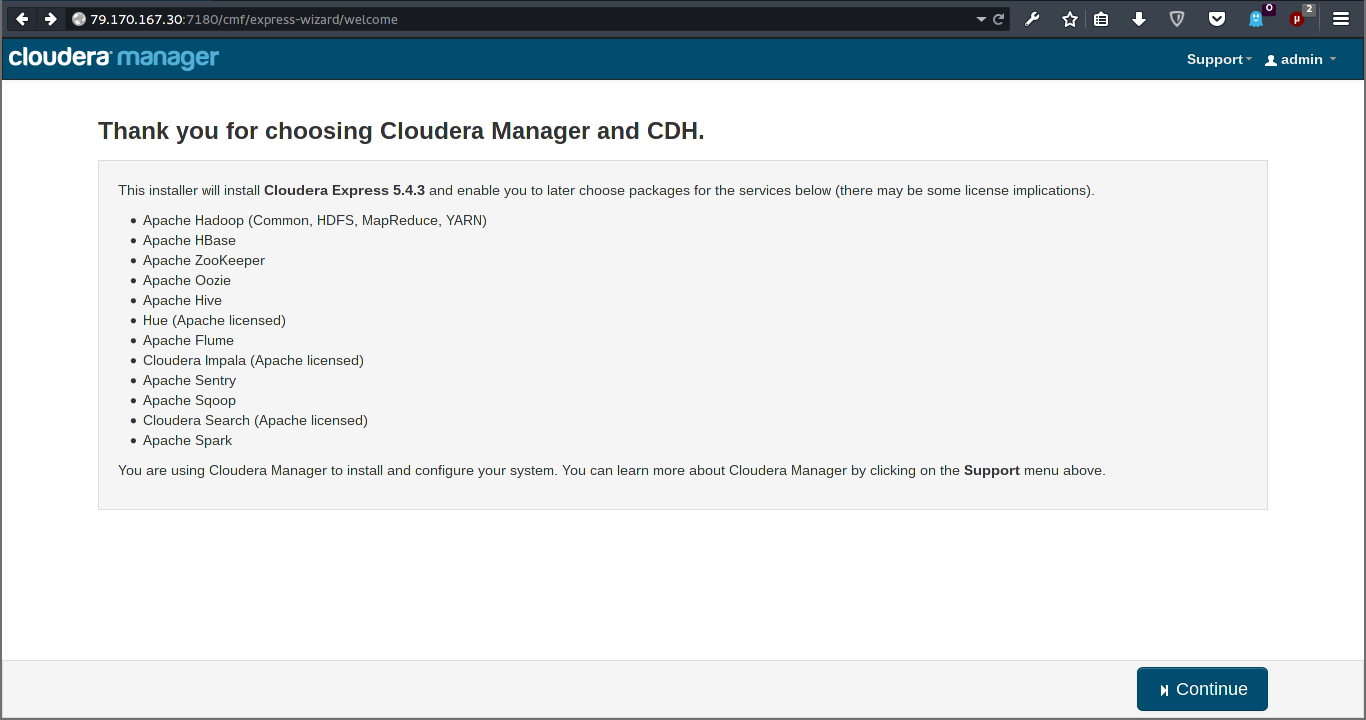
\includegraphics[width=1.0\textwidth]{image-000}
\end{figure}

\newpage

\begin{figure}[ht!]
    \center
    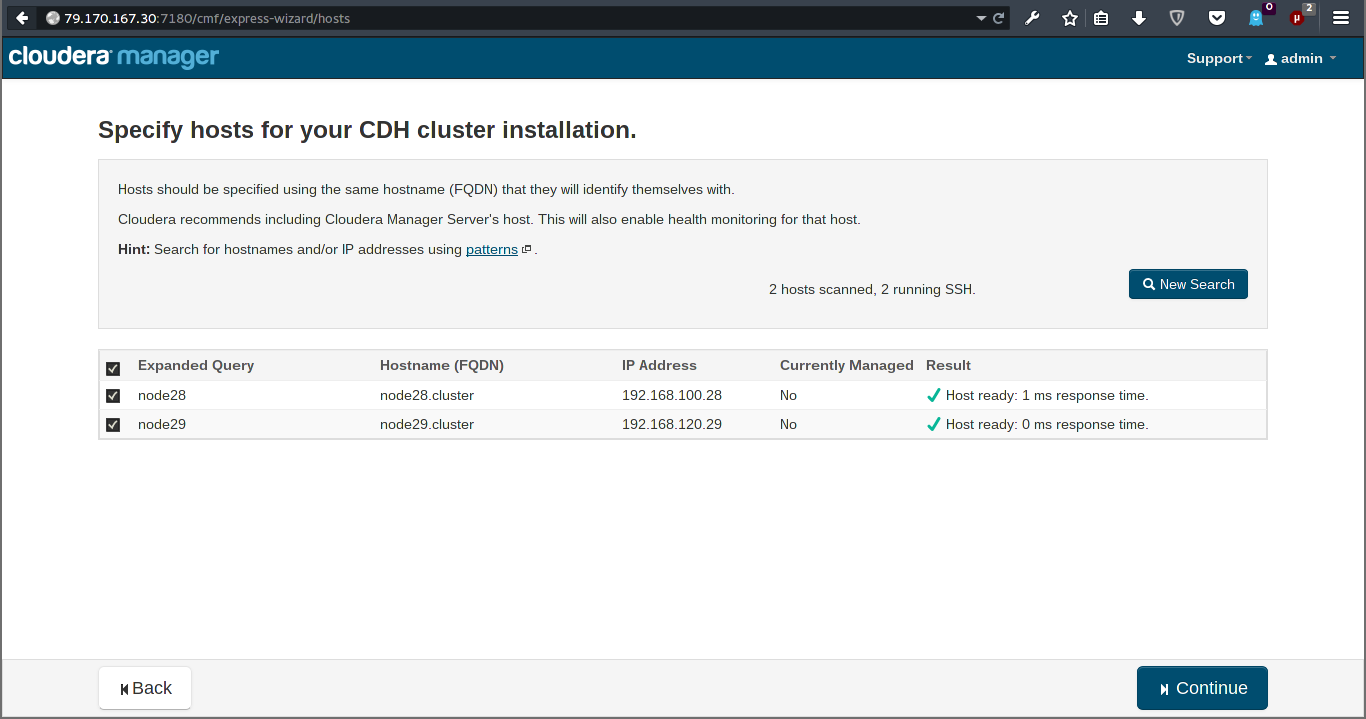
\includegraphics[width=1.0\textwidth]{image-001}
    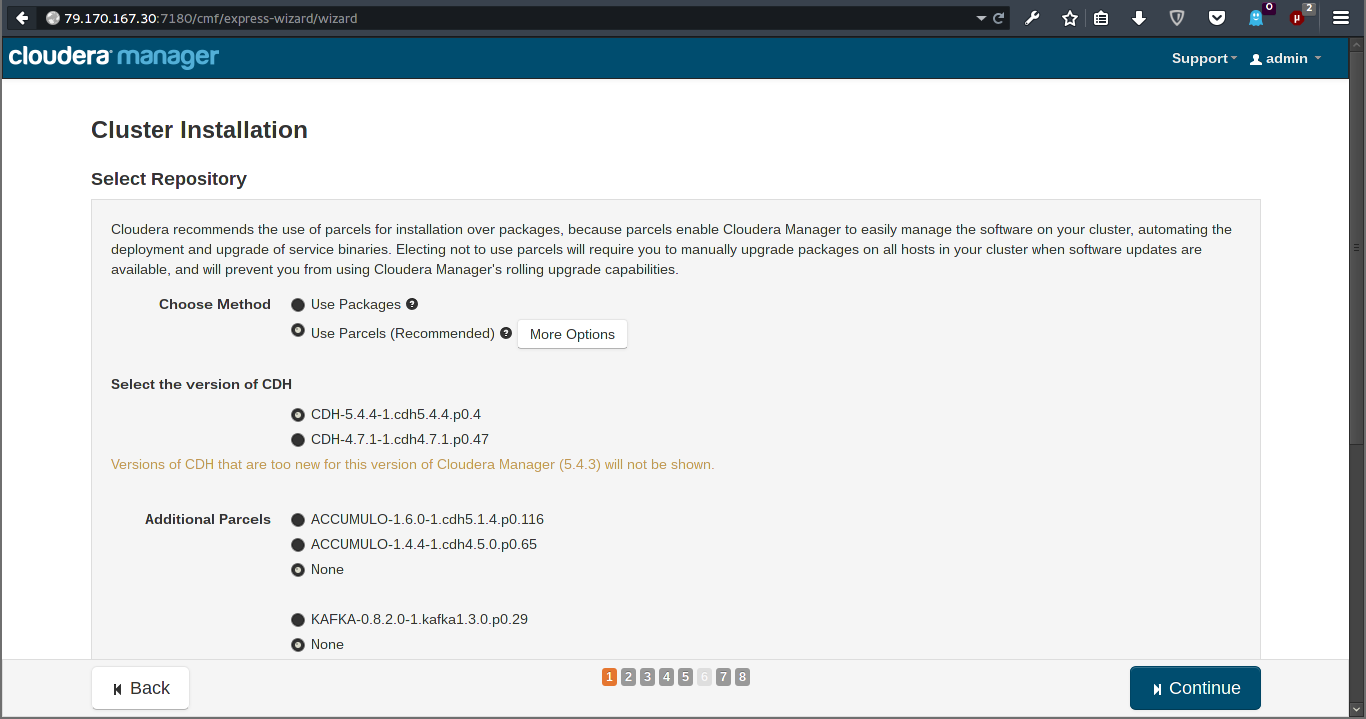
\includegraphics[width=1.0\textwidth]{image-002}
\end{figure}

\newpage

\begin{figure}[ht!]
    \center
    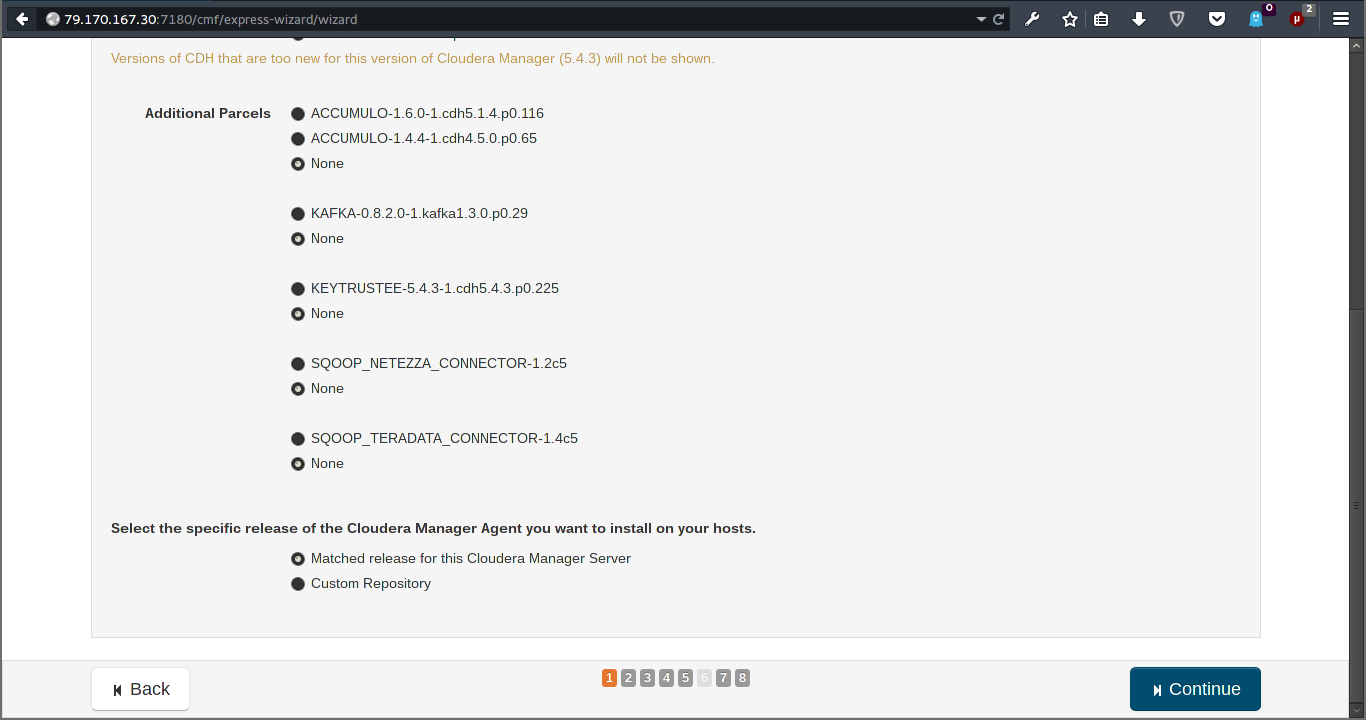
\includegraphics[width=1.0\textwidth]{image-003}
    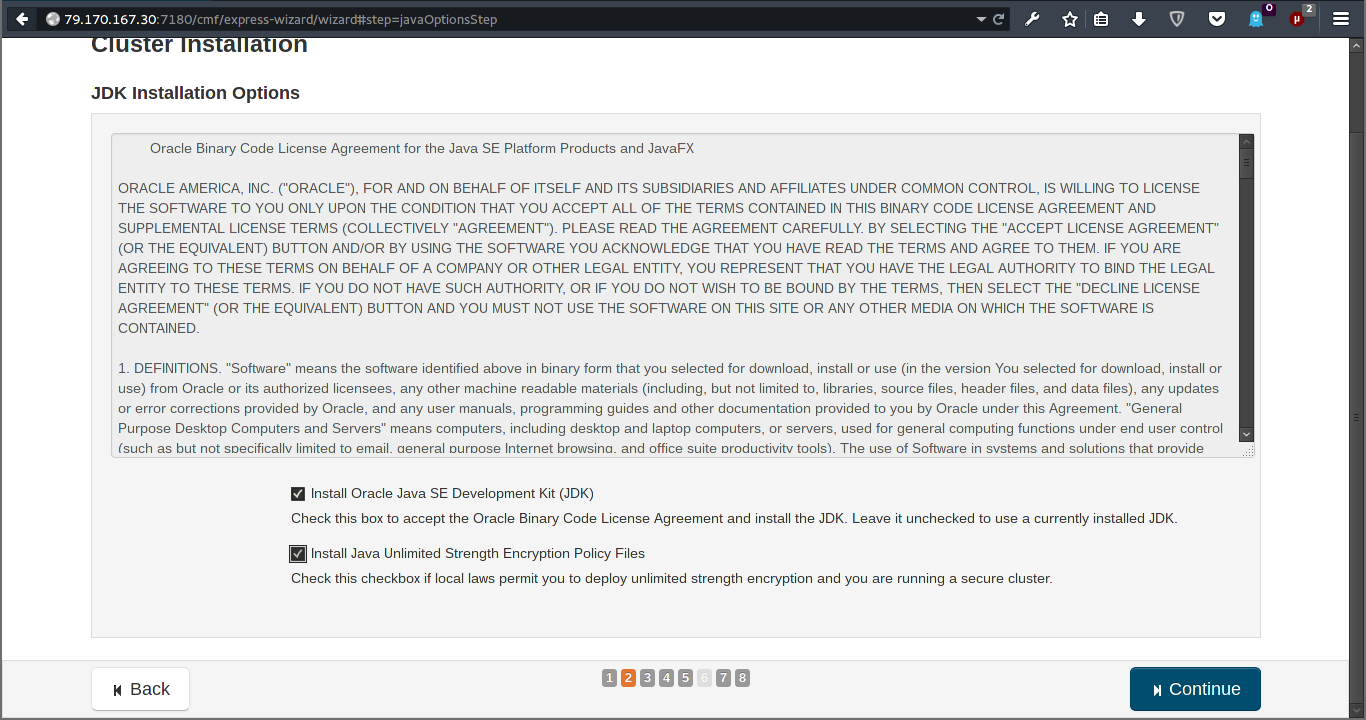
\includegraphics[width=1.0\textwidth]{image-004}
\end{figure}

\newpage

\begin{figure}[ht!]
    \center
    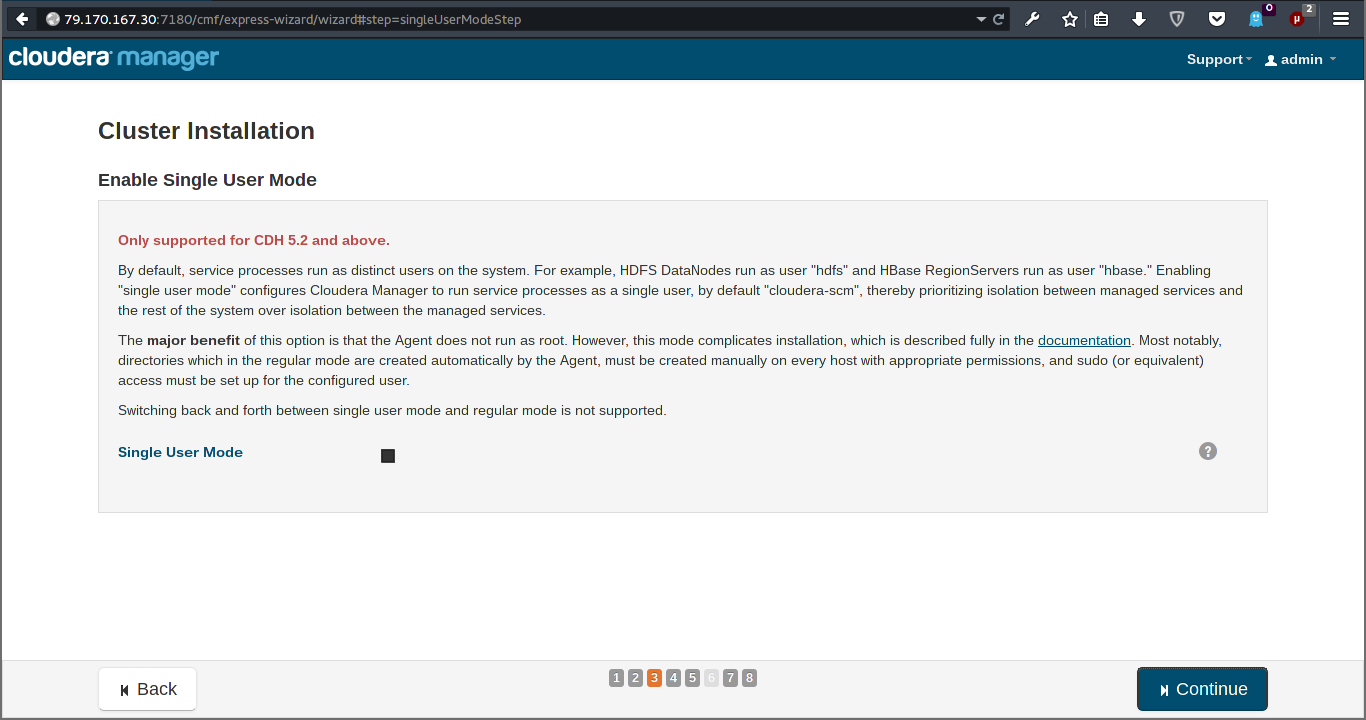
\includegraphics[width=1.0\textwidth]{image-005}
    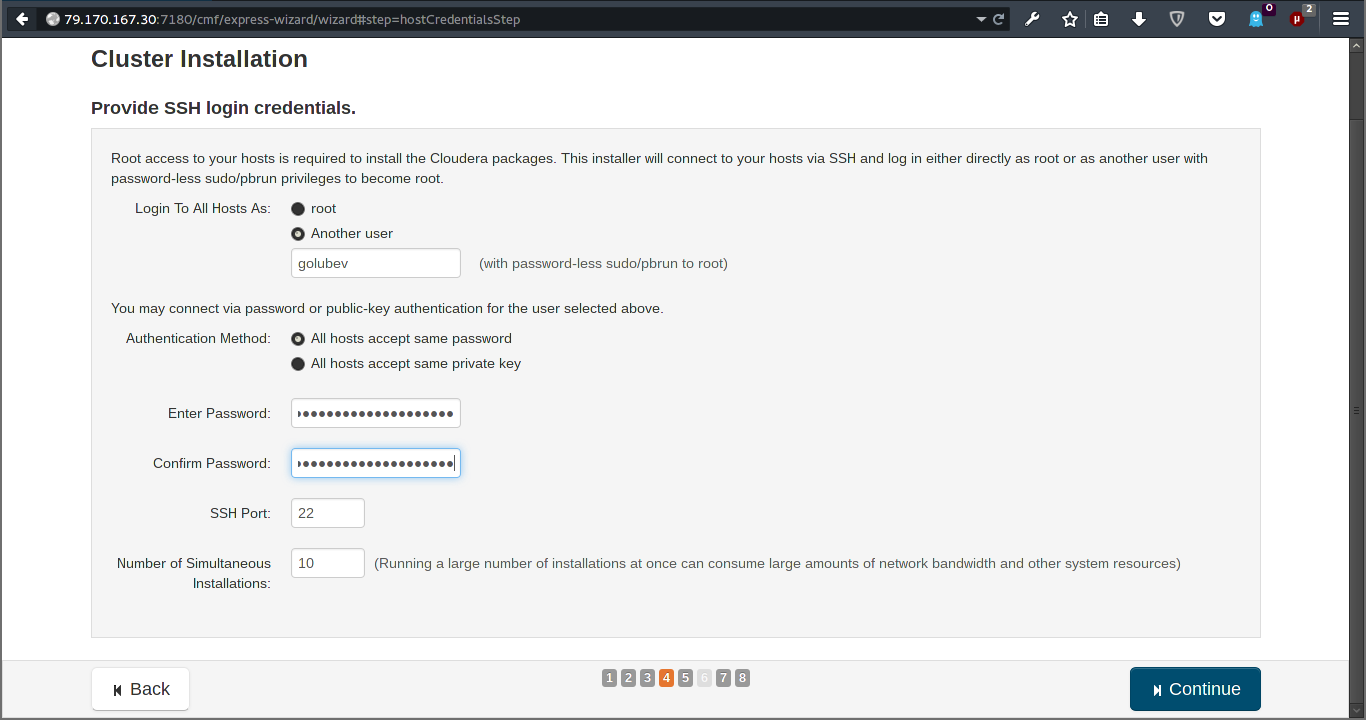
\includegraphics[width=1.0\textwidth]{image-006}
\end{figure}

\newpage

\begin{figure}[ht!]
    \center
    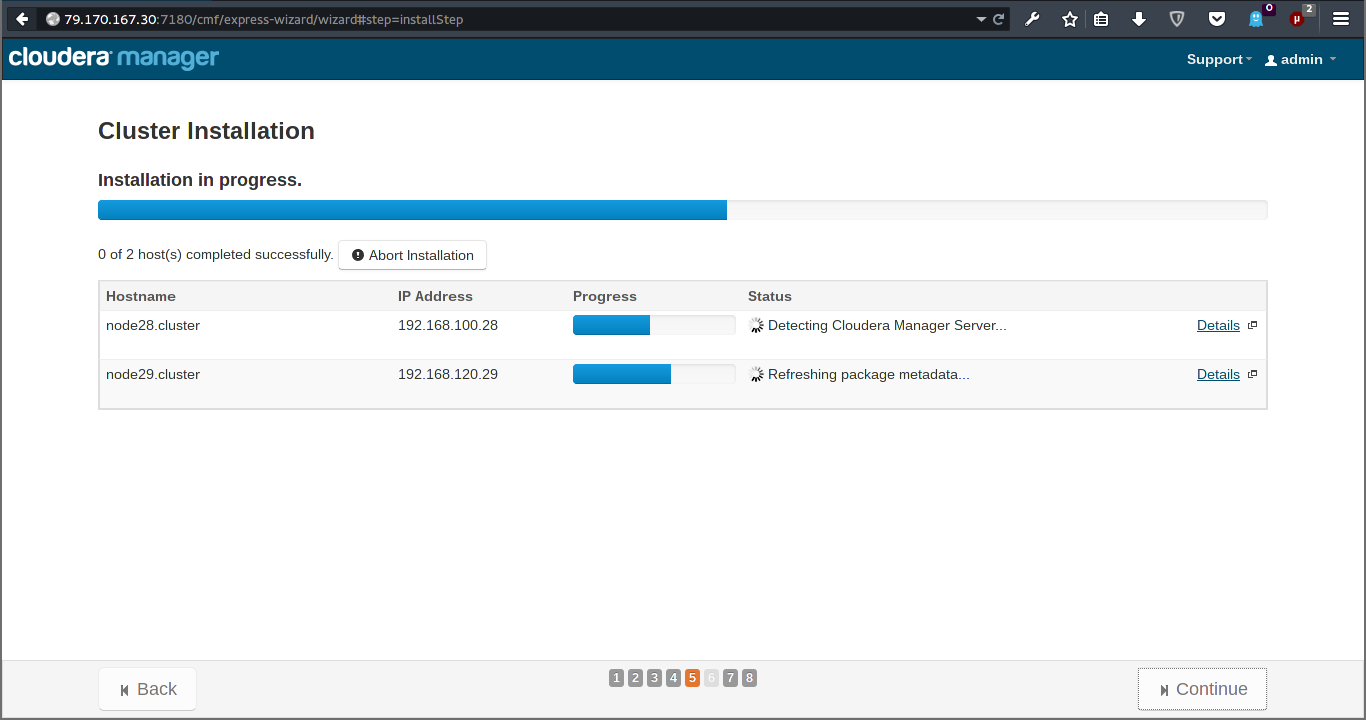
\includegraphics[width=1.0\textwidth]{image-007}
    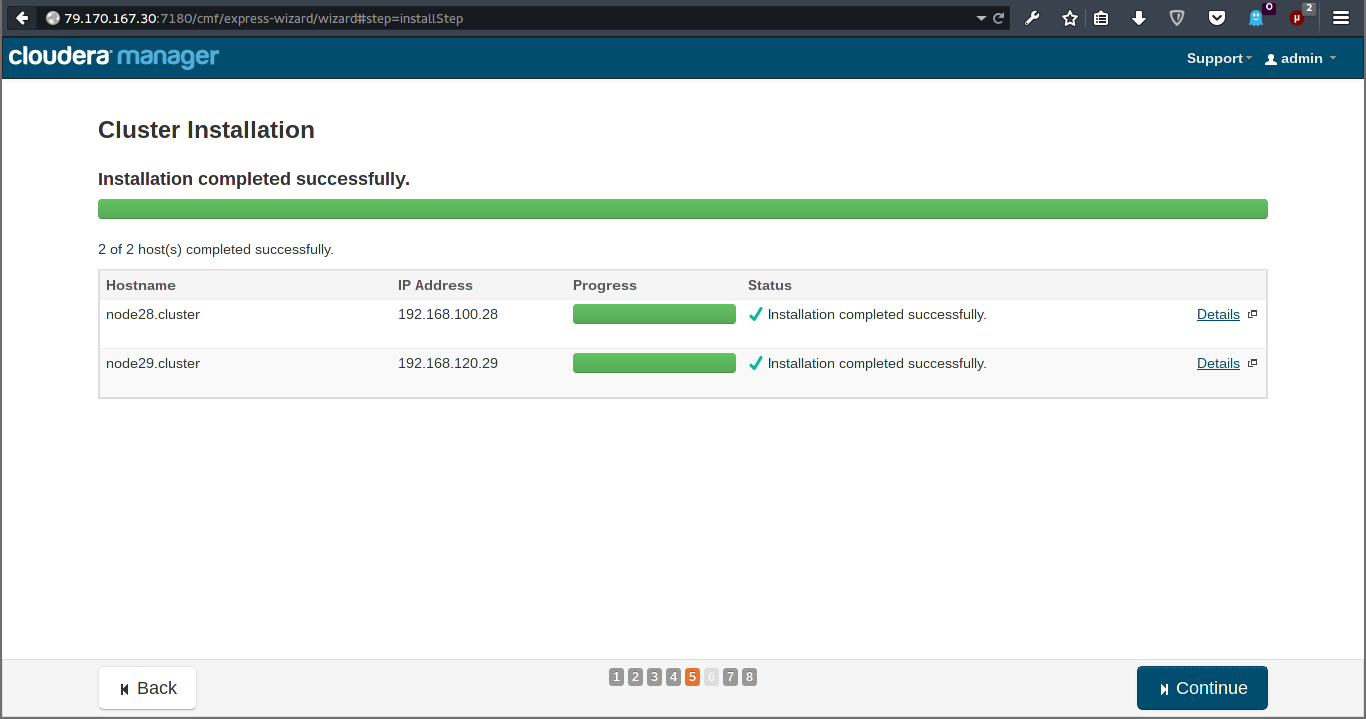
\includegraphics[width=1.0\textwidth]{image-008}
\end{figure}

В случае если каталог \emph{/opt} для всех нод является одним, то нужно произвести следующие действия.

Создадим несколько каталогов в \emph{/hadoop/}
\begin{lstlisting}
$ sudo mkdir /hadoop/cloudera/csd
$ sudo /hadoop/cloudera/parcel-cache
$ sudo mkdir /hadop/cloudera/parcel-repo
$ sudo /hadoop/cloudera/parcels
\end{lstlisting}
И редактируем файл \emph{/etc/cloudera-scm-agent/config.ini} на каждой ноде, а потом перезапускаем сервис
\begin{lstlisting}
$ sudo vim /etc/cloudera-scm-agent/config.ini
parcel_dir=/hadoop/cloudera/parcels
$ sudo service cloudera-scm-agent restart
\end{lstlisting}
Подробнее можно почитать по следующей ссылке \url{http://www.cloudera.com/content/cloudera/en/documentation/cloudera-manager/v4-7-3/Cloudera-Manager-Release-Notes/cmrn_fixed_in_4_7_2.html}

Далее в браузере щёлкаем по значку Cloudera Manager и переходим во вкладку Hosts->Configuration, где 
устанавливаем следующие параметры
\begin{itemize}
    \item Parcel Directory
    \item Local Parcel Repository Path
\end{itemize}
как на скриншотах

\begin{figure}[ht!]
    \center
    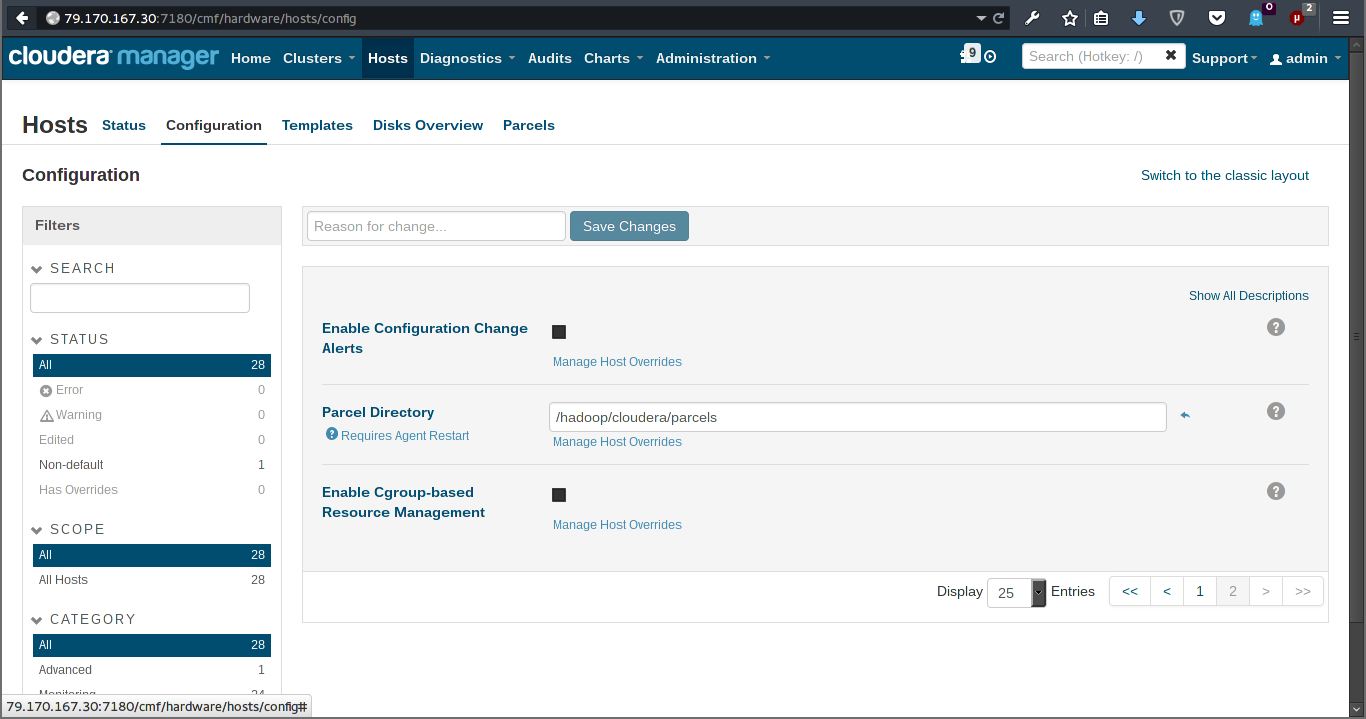
\includegraphics[width=1.0\textwidth]{image-009}
\end{figure}

\newpage

\begin{figure}[ht!]
    \center
    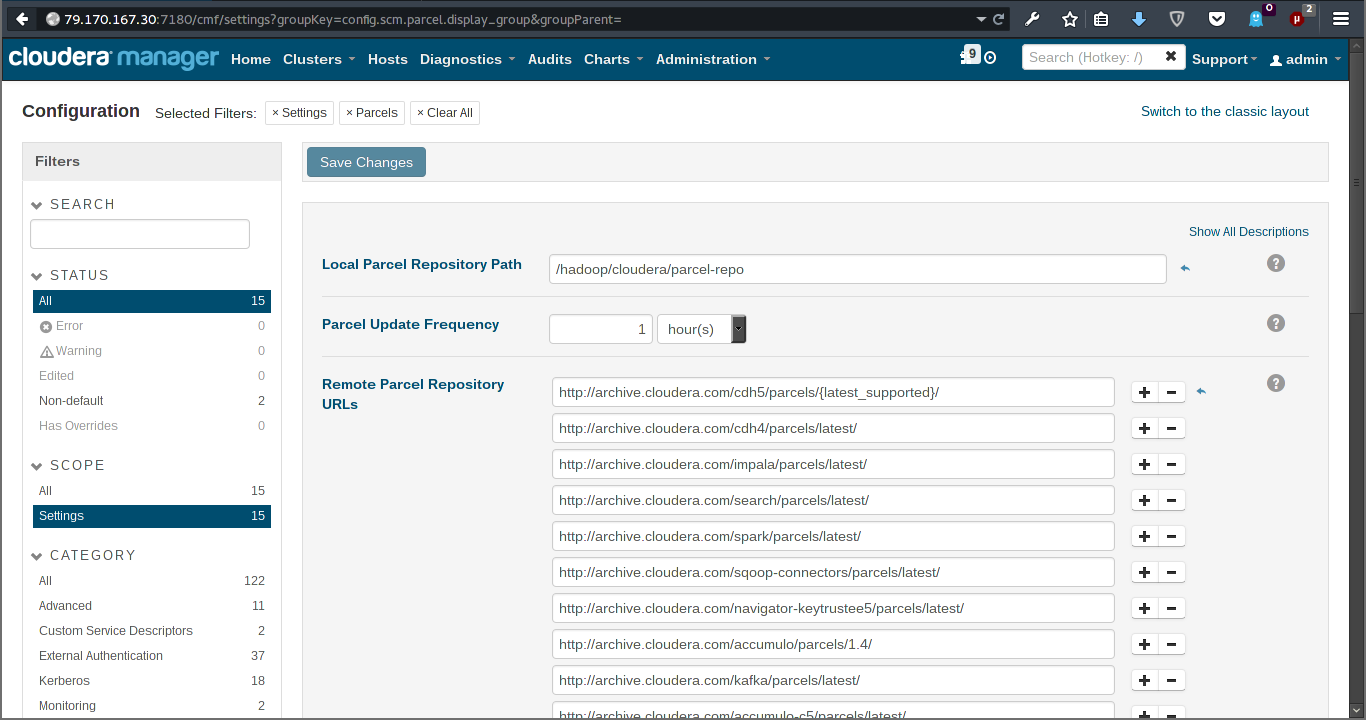
\includegraphics[width=1.0\textwidth]{image-010}
    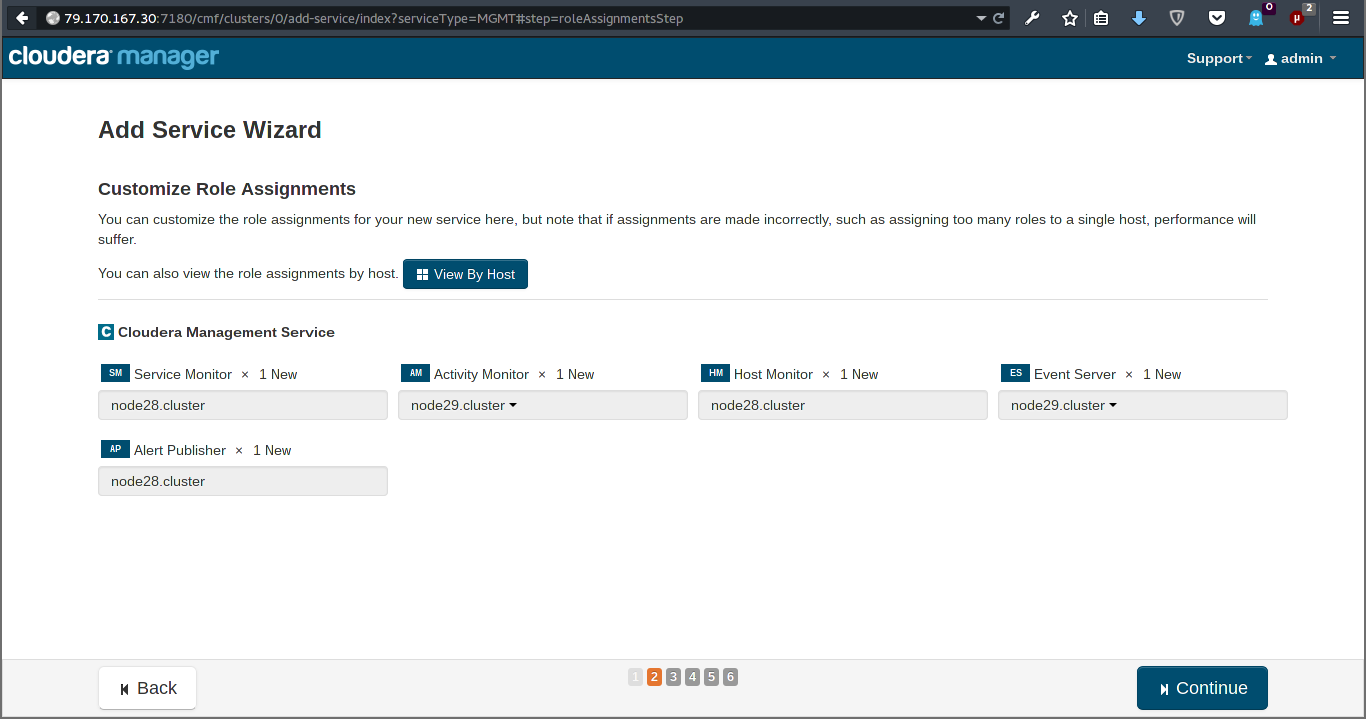
\includegraphics[width=1.0\textwidth]{image-011}
\end{figure}
А далее переходим на главную и нажимает кнопку \emph{Add Service} и продолжаем установку.

\newpage

\begin{figure}[ht!]
    \center
    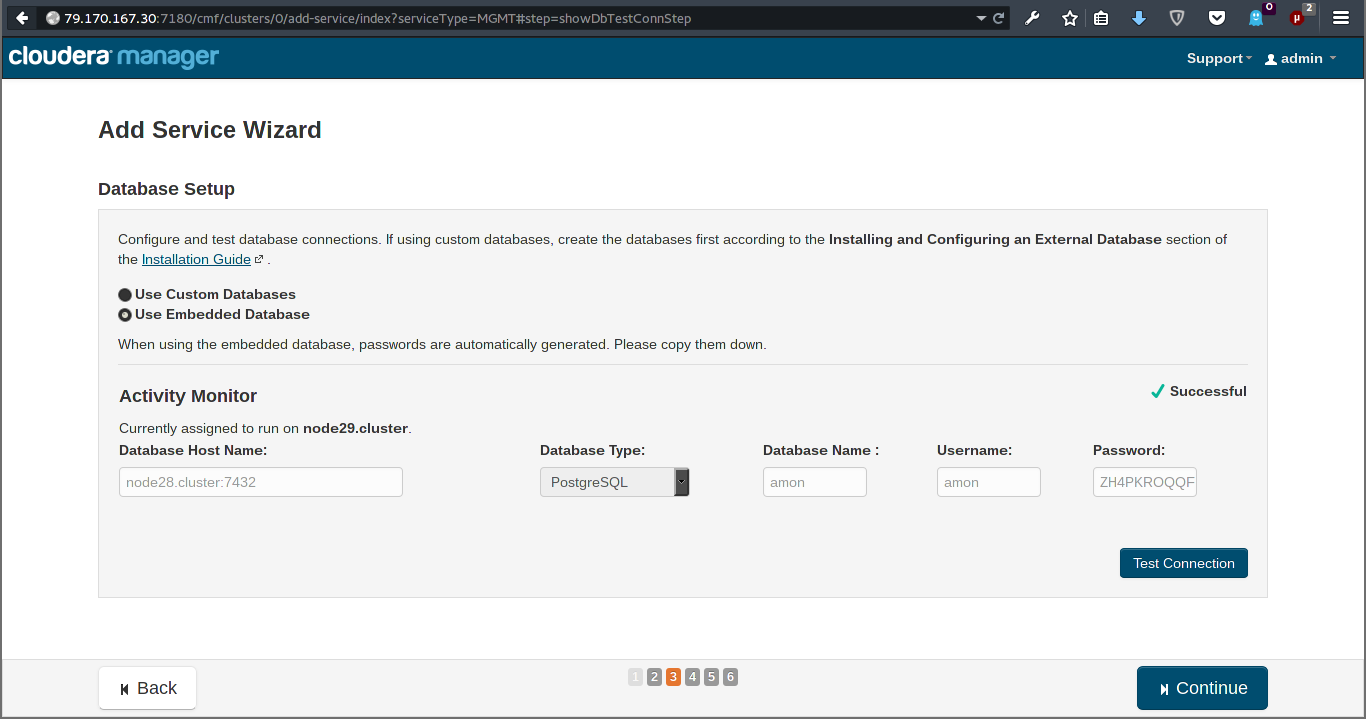
\includegraphics[width=1.0\textwidth]{image-012}
    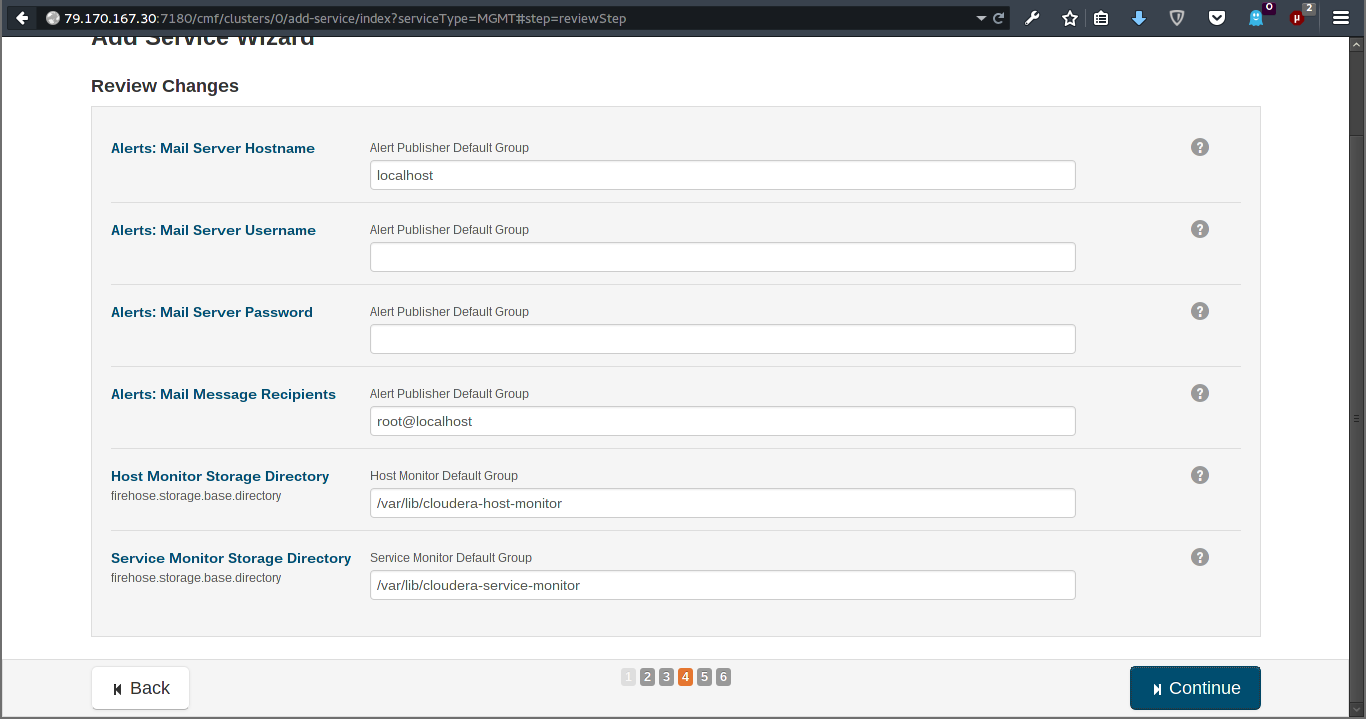
\includegraphics[width=1.0\textwidth]{image-013}
\end{figure}

\newpage

\begin{figure}[ht!]
    \center
    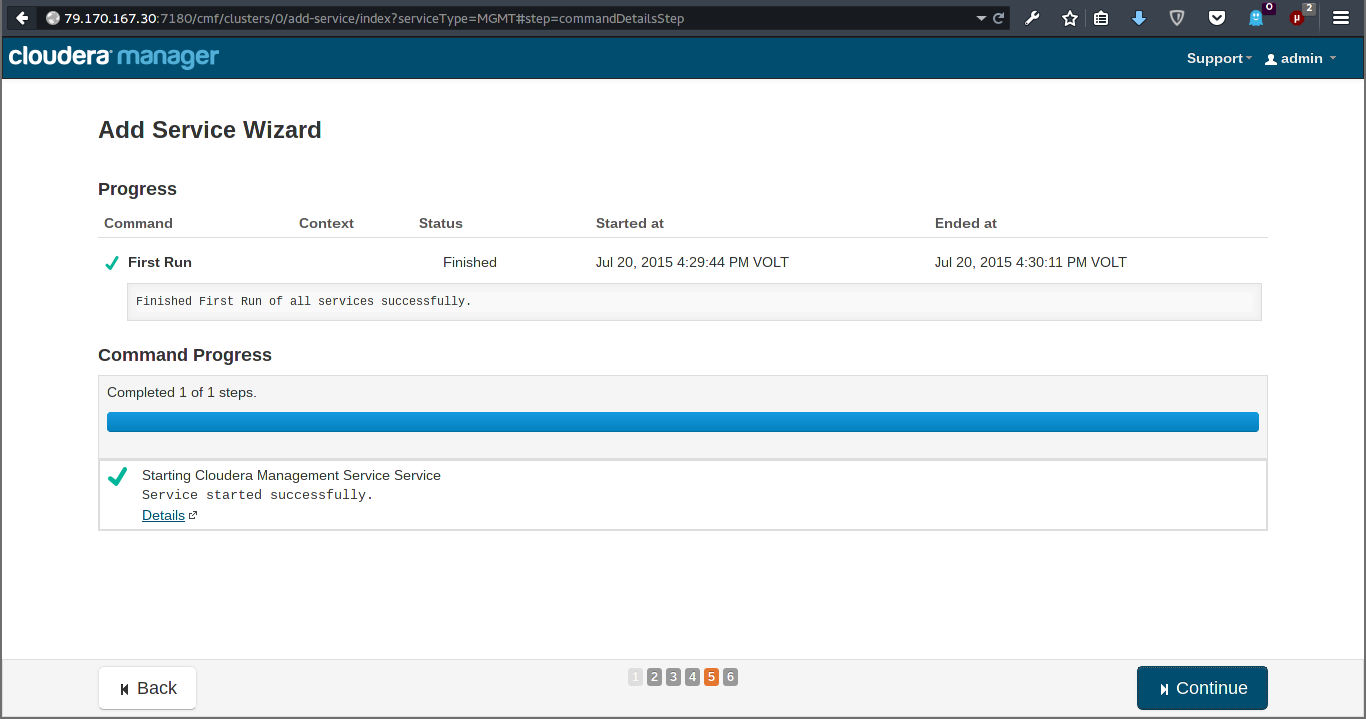
\includegraphics[width=1.0\textwidth]{image-014}
\end{figure}

Если вы дошли до этого шага изменяя параметры \emph{Parcel Directory}, то выйдете на главную страницу и 
нажмите на кнопку \emph{Add cluster} и выберите параметры, которые были уже раньше. Далее идёт установка 
основных пакетов (она может длиться значительное время).

\begin{figure}[ht!]
    \center
    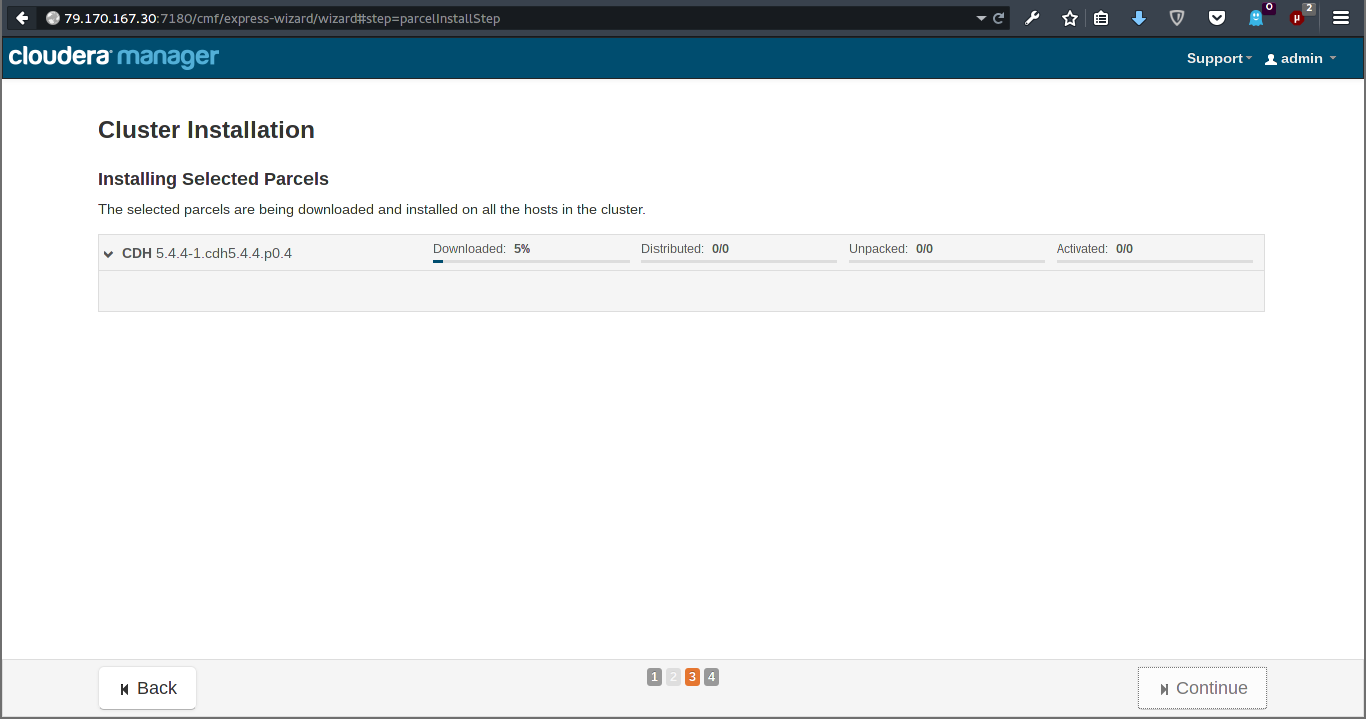
\includegraphics[width=1.0\textwidth]{image-020}
\end{figure}

\newpage

\begin{figure}[ht!]
    \center
    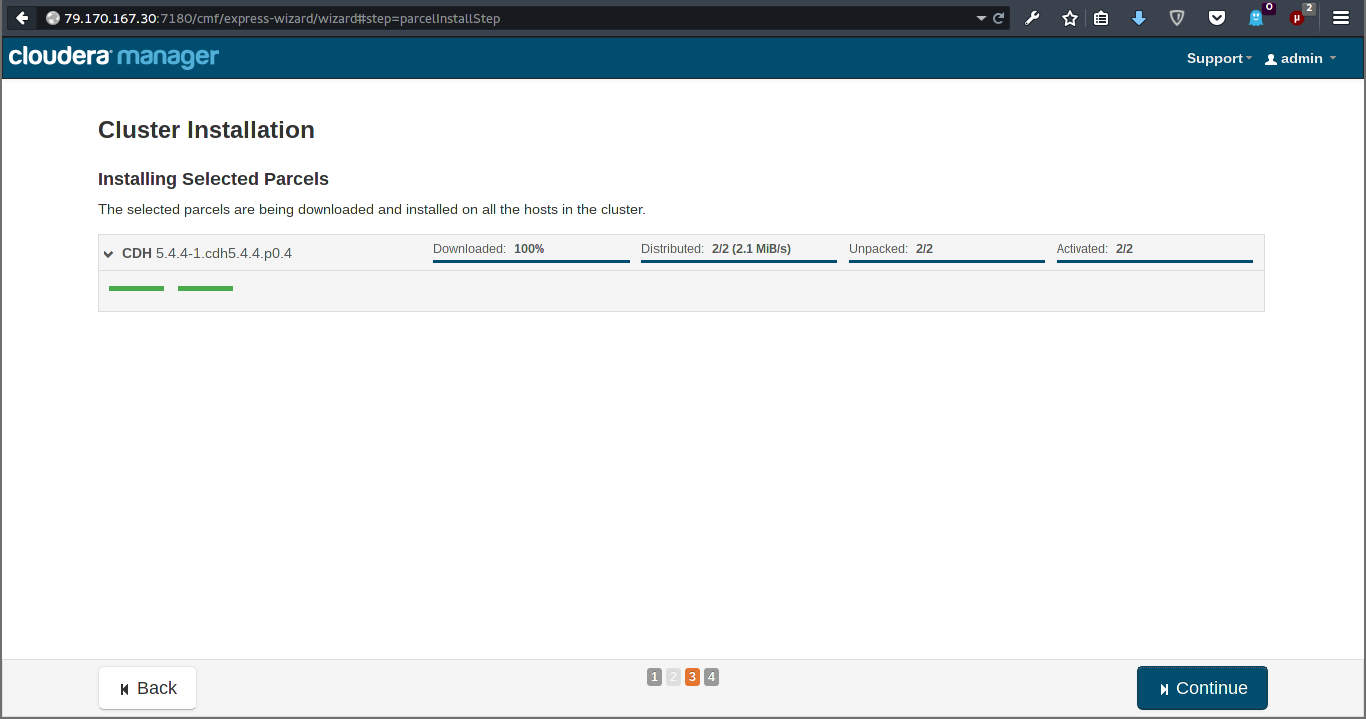
\includegraphics[width=1.0\textwidth]{image-021}
    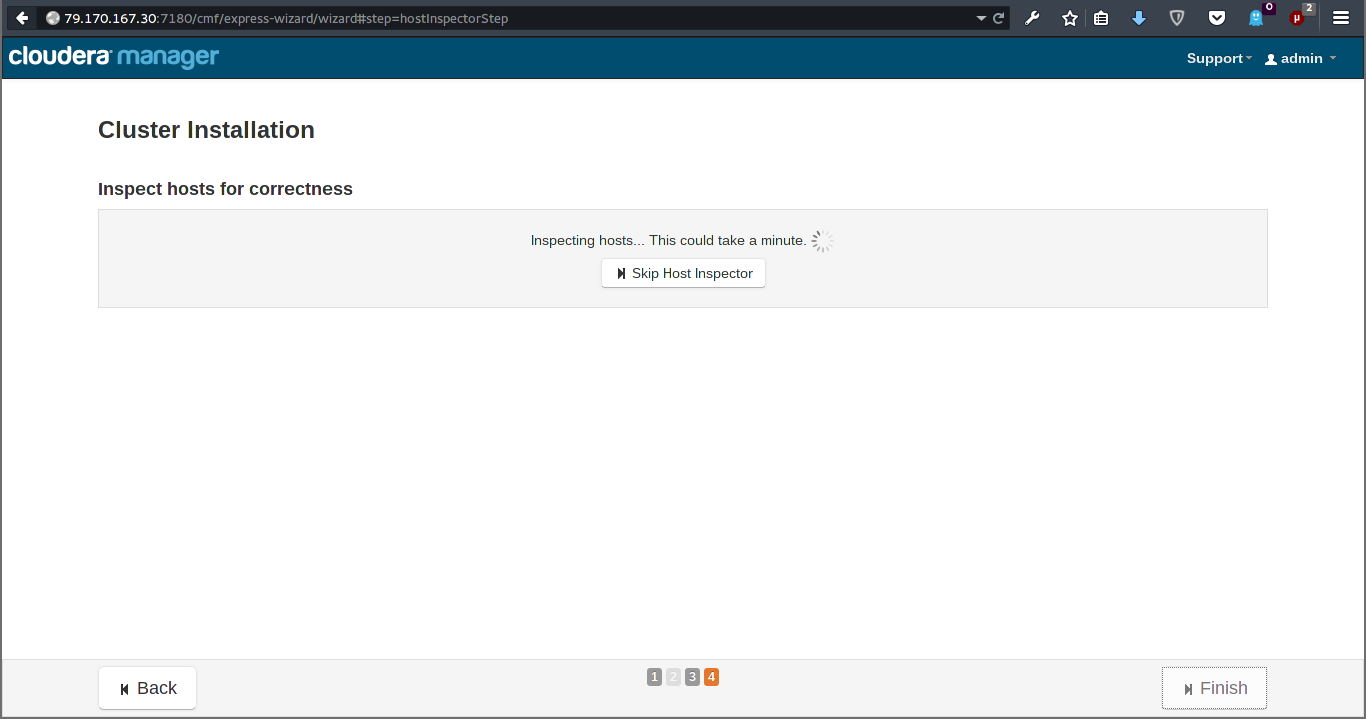
\includegraphics[width=1.0\textwidth]{image-022}
\end{figure}


\newpage

\begin{figure}[ht!]
    \center
    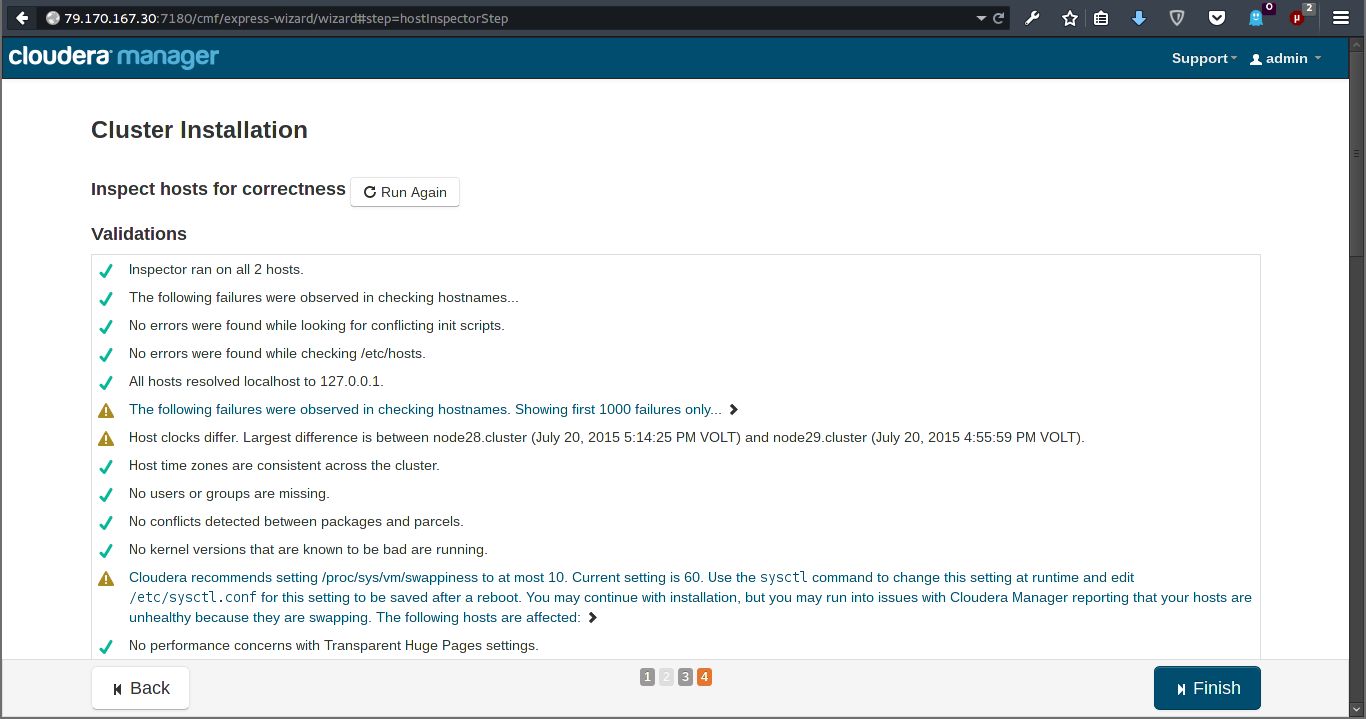
\includegraphics[width=1.0\textwidth]{image-023}
    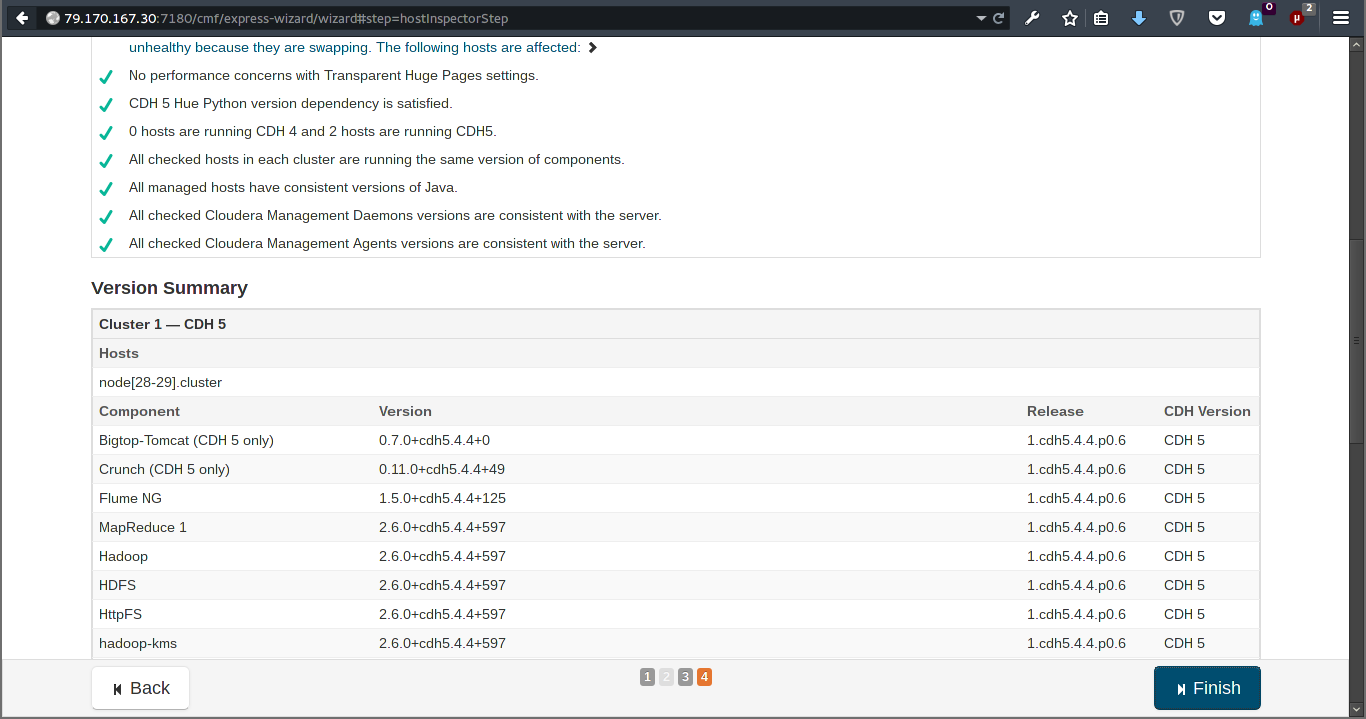
\includegraphics[width=1.0\textwidth]{image-024}
\end{figure}

\newpage

\begin{figure}[ht!]
    \center
    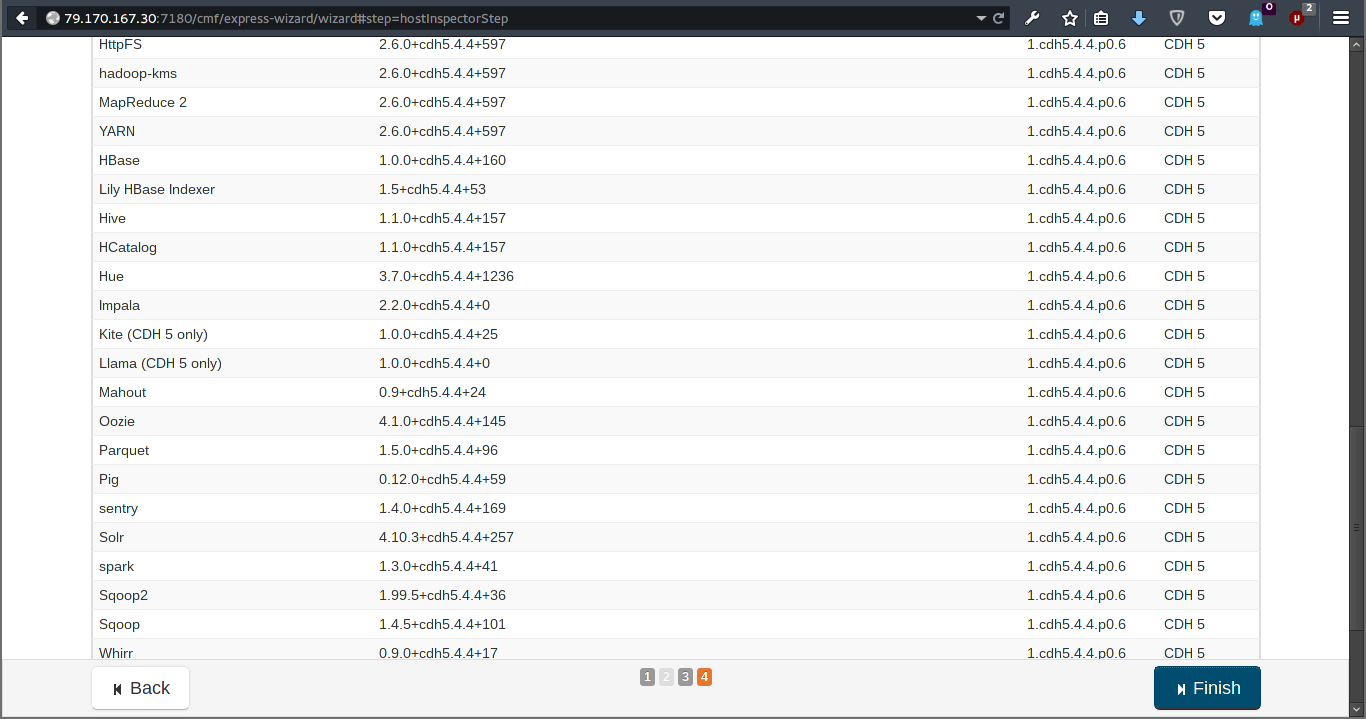
\includegraphics[width=1.0\textwidth]{image-025}
    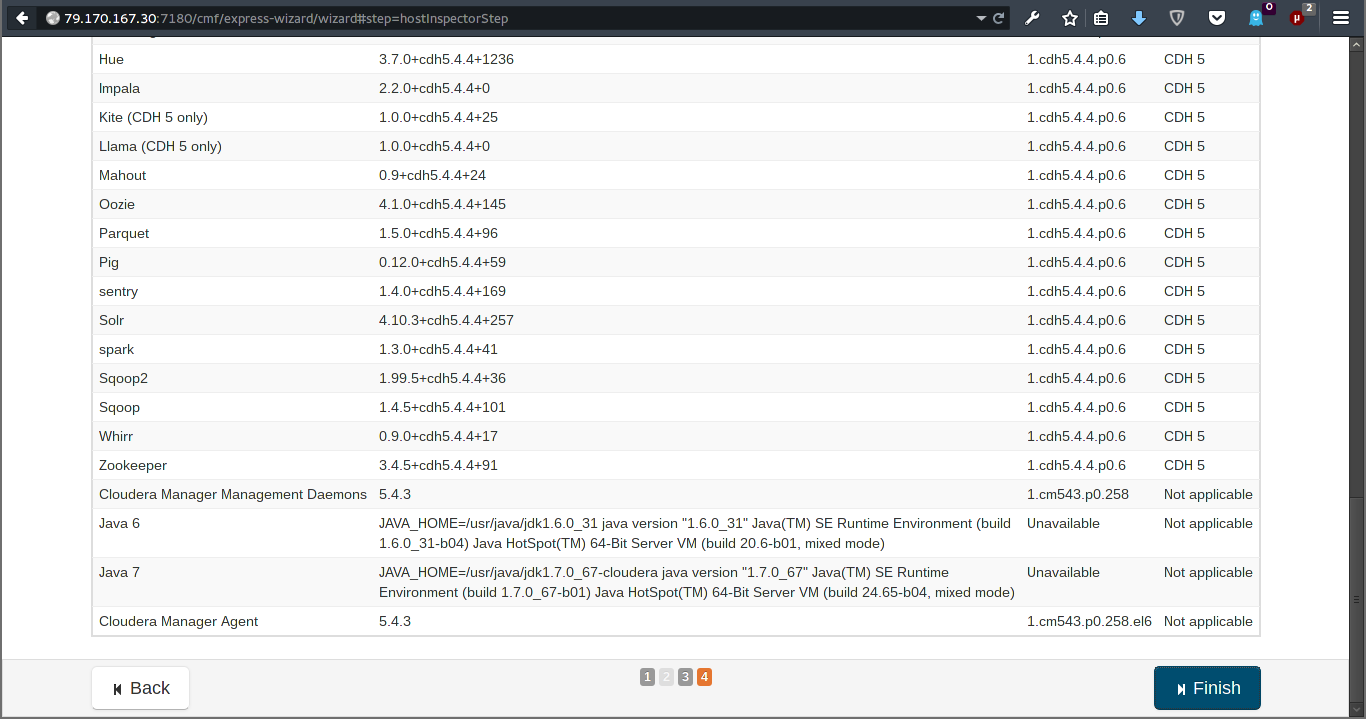
\includegraphics[width=1.0\textwidth]{image-026}
\end{figure}

\newpage

\begin{figure}[ht!]
    \center
    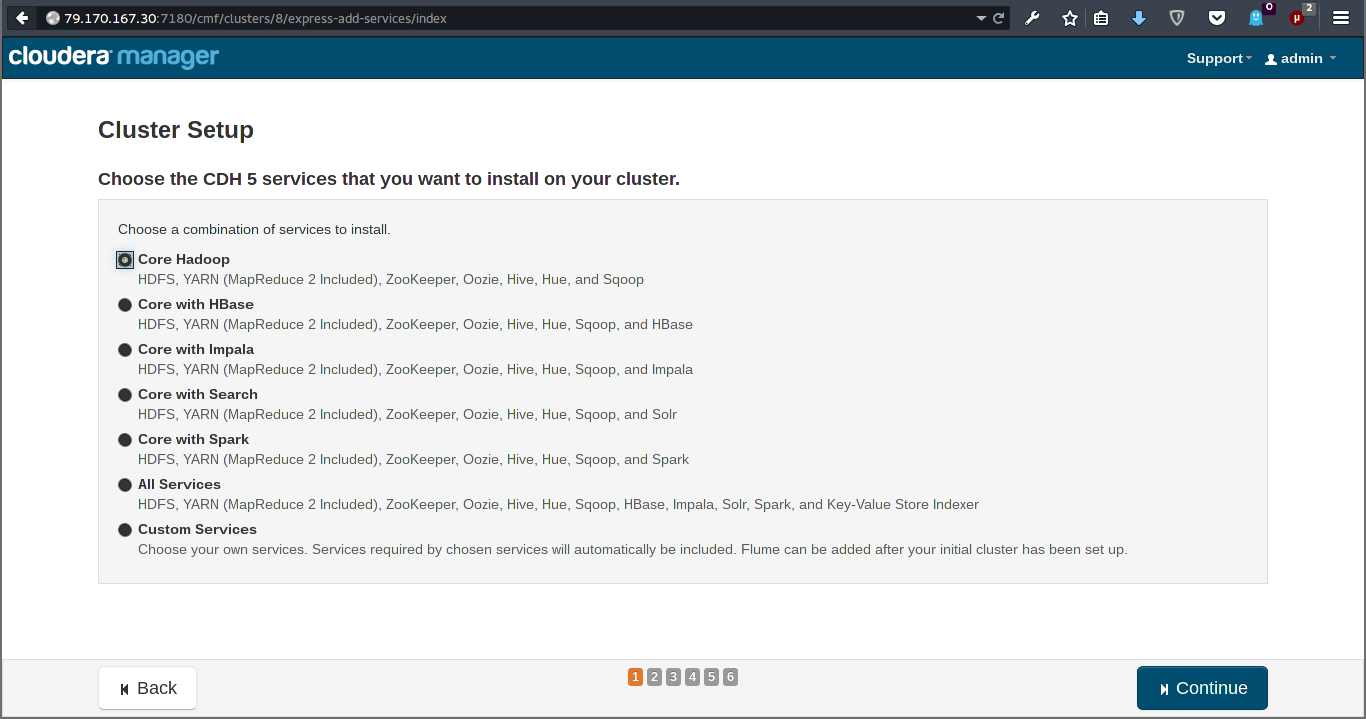
\includegraphics[width=1.0\textwidth]{image-027}
    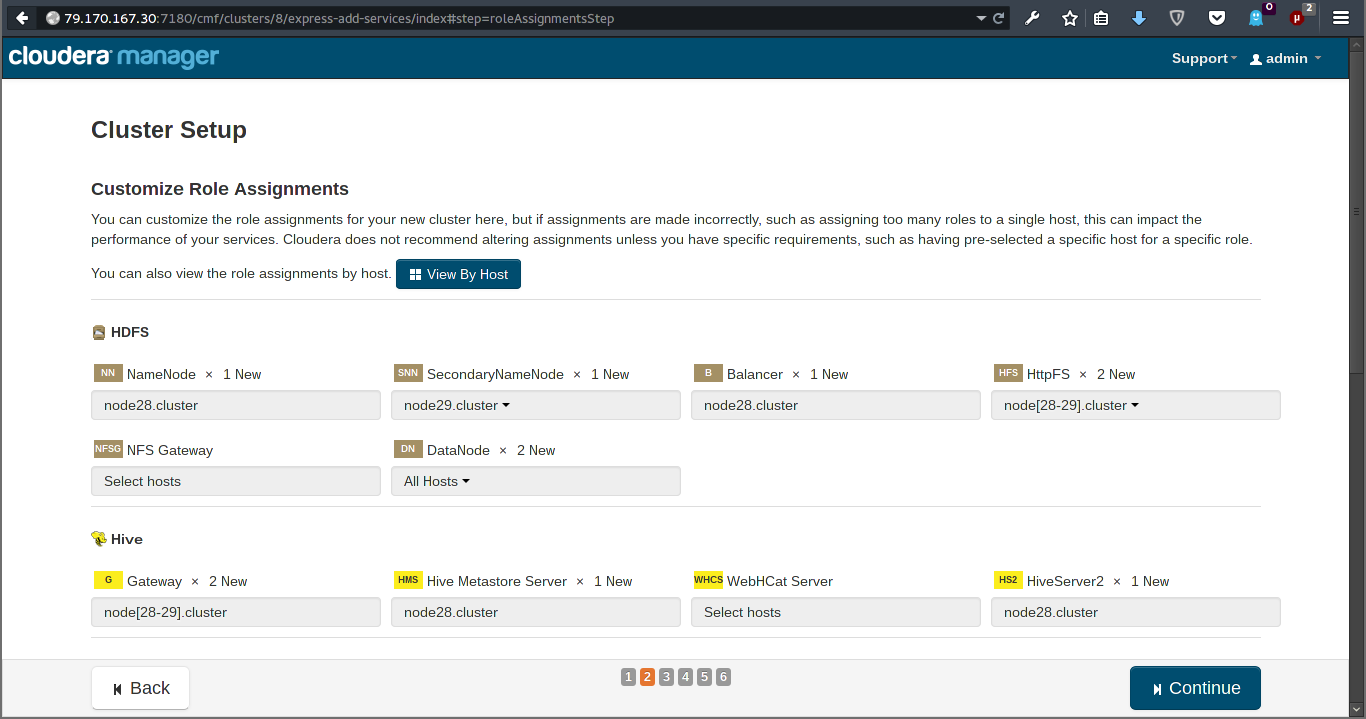
\includegraphics[width=1.0\textwidth]{image-028}
\end{figure}

\newpage

\begin{figure}[ht!]
    \center
    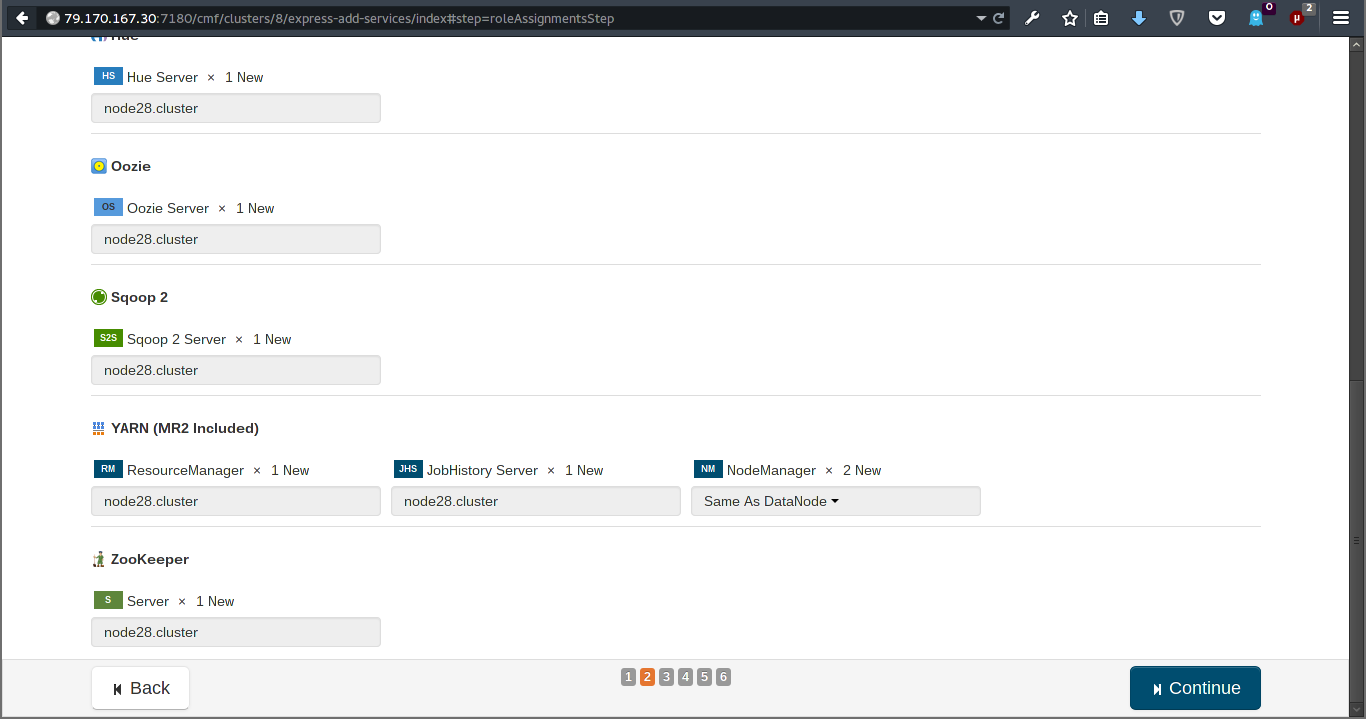
\includegraphics[width=1.0\textwidth]{image-029}
    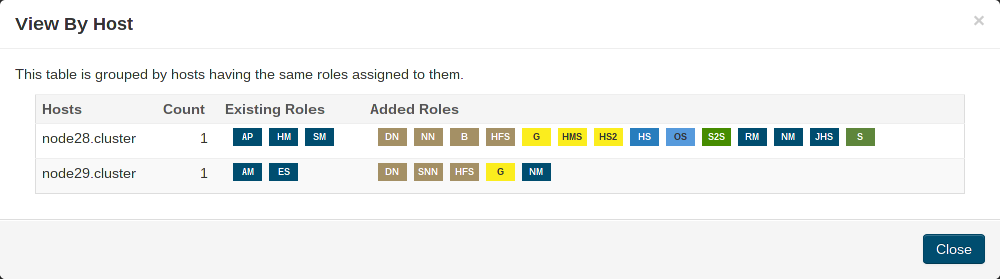
\includegraphics[width=1.0\textwidth]{image-030}
    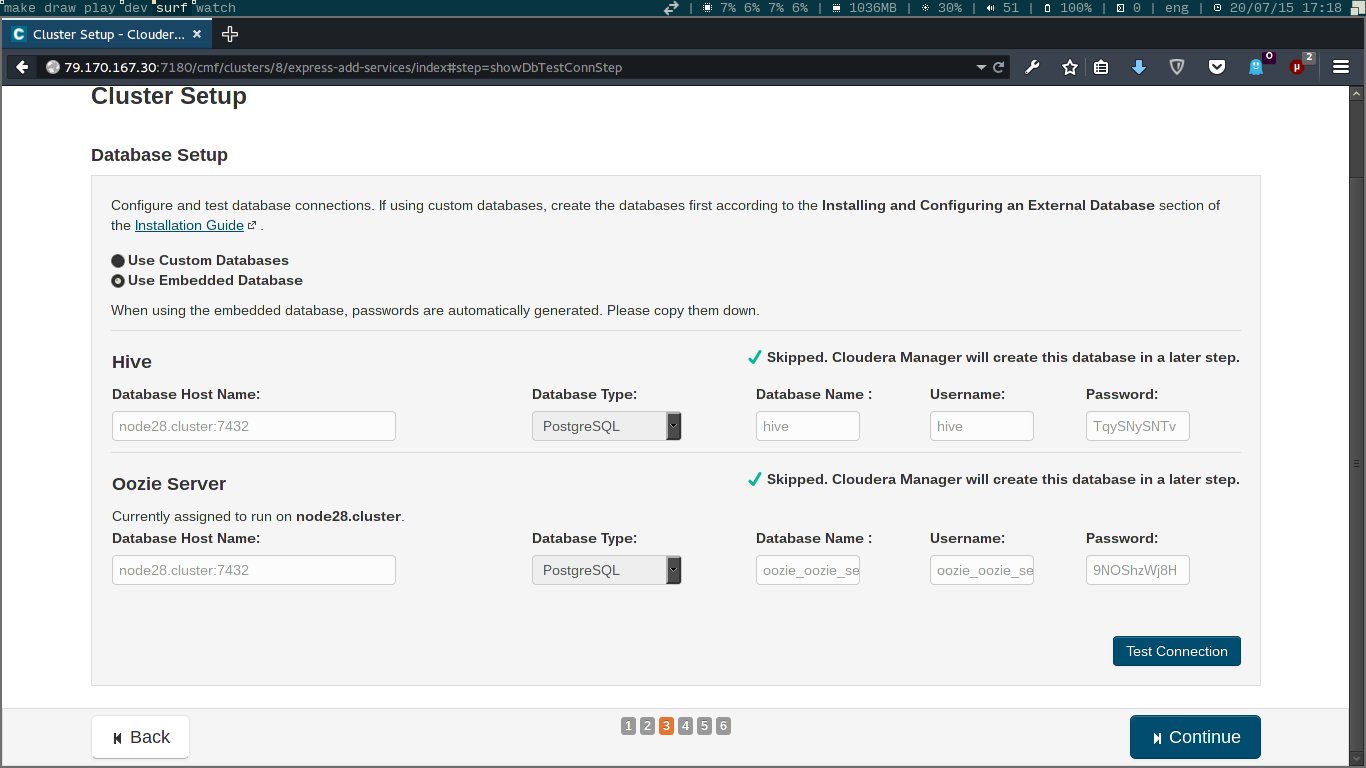
\includegraphics[width=1.0\textwidth]{image-031}
\end{figure}

\newpage

\begin{figure}[ht!]
    \center
    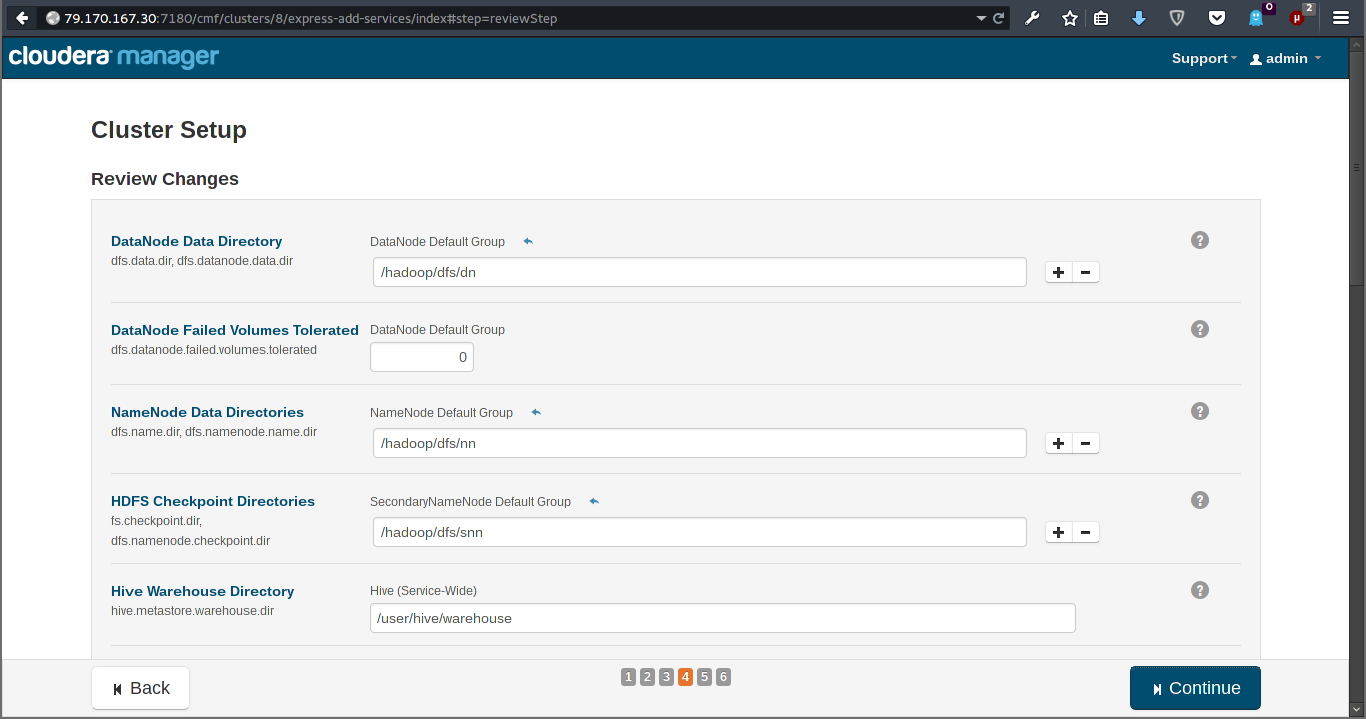
\includegraphics[width=1.0\textwidth]{image-032}
    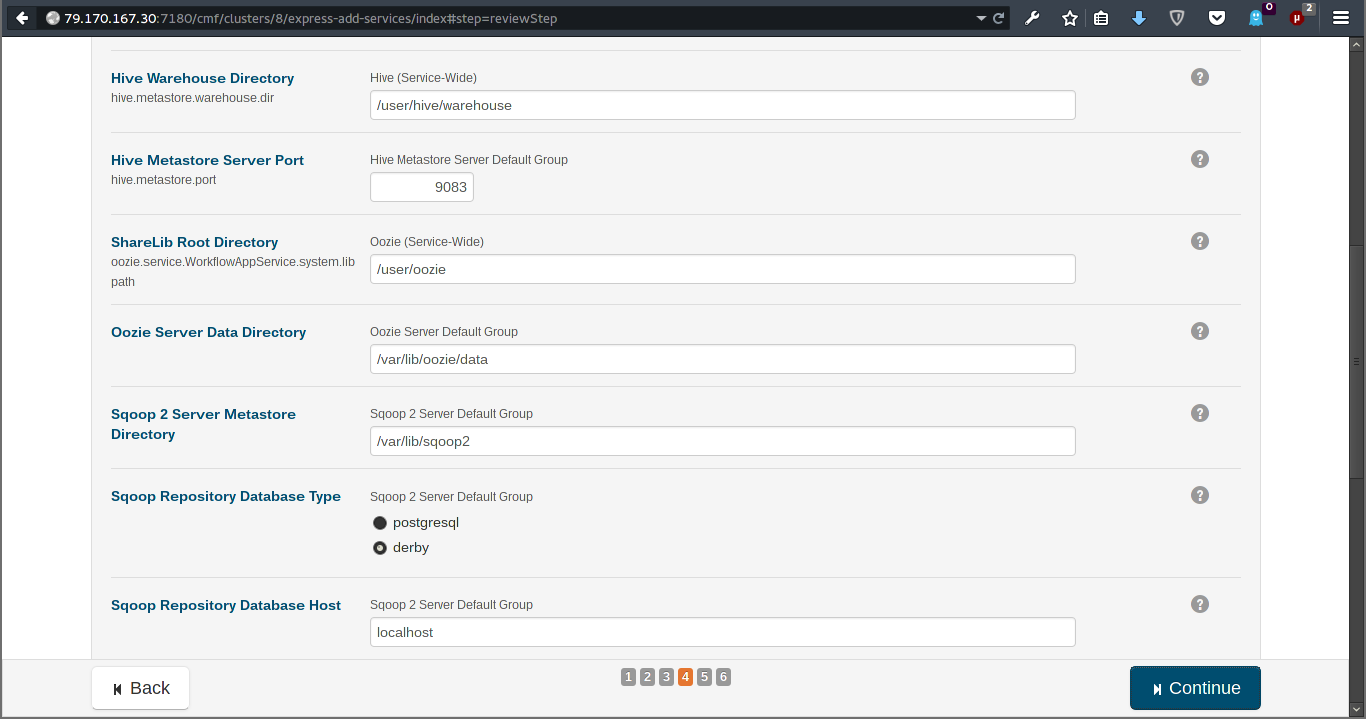
\includegraphics[width=1.0\textwidth]{image-033}
\end{figure}

\newpage

\begin{figure}[ht!]
    \center
    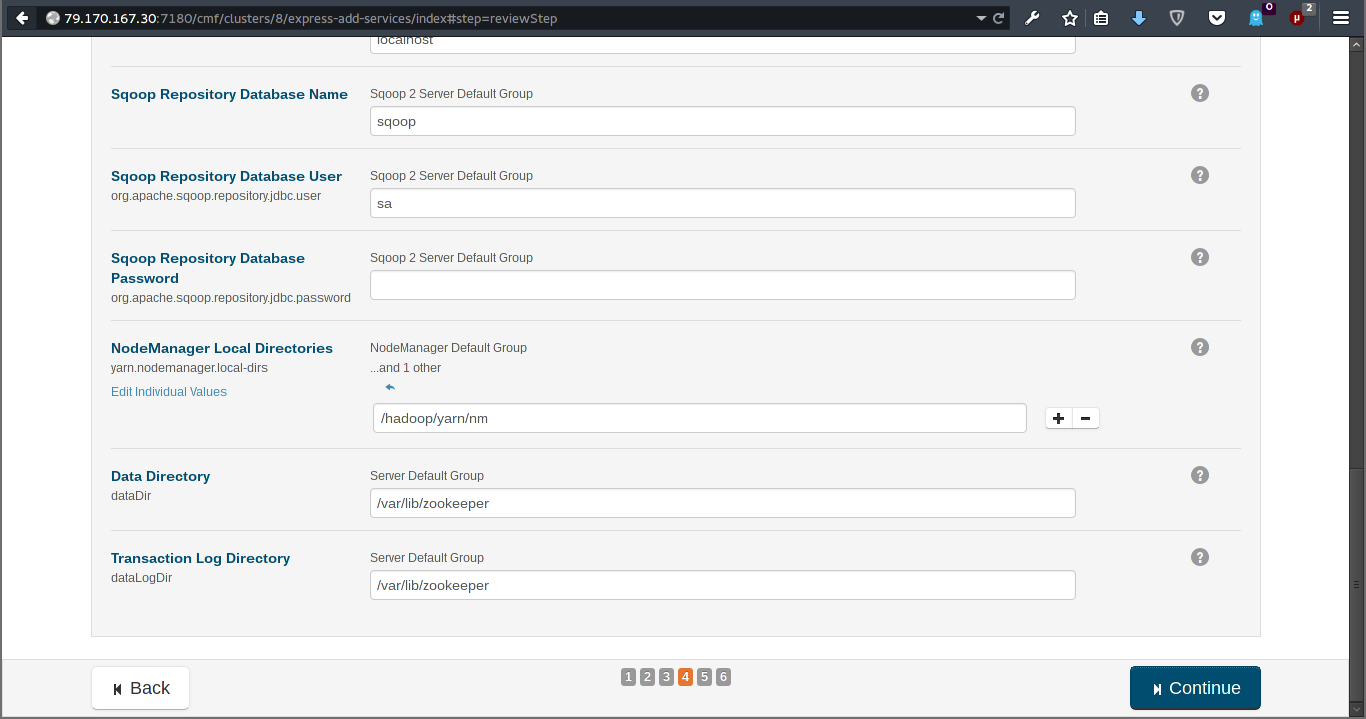
\includegraphics[width=1.0\textwidth]{image-034}
    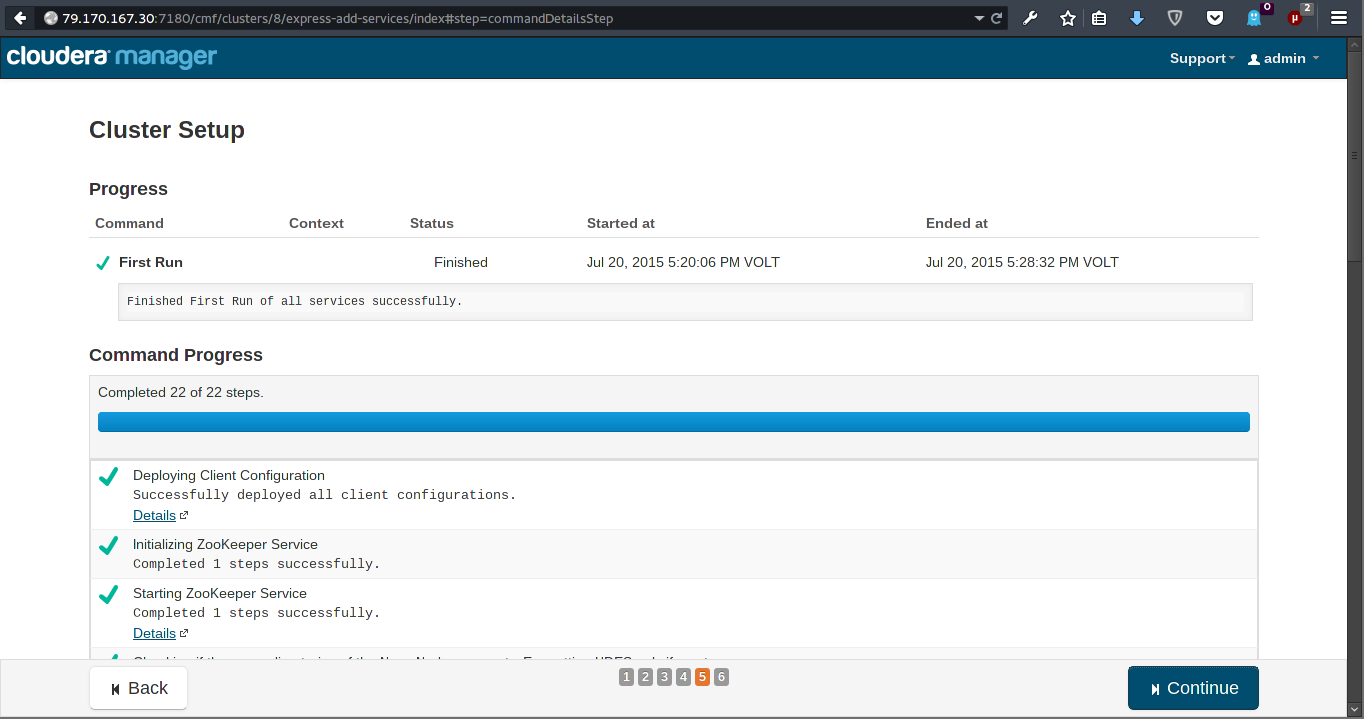
\includegraphics[width=1.0\textwidth]{image-035}
\end{figure}

\newpage

\begin{figure}[ht!]
    \center
    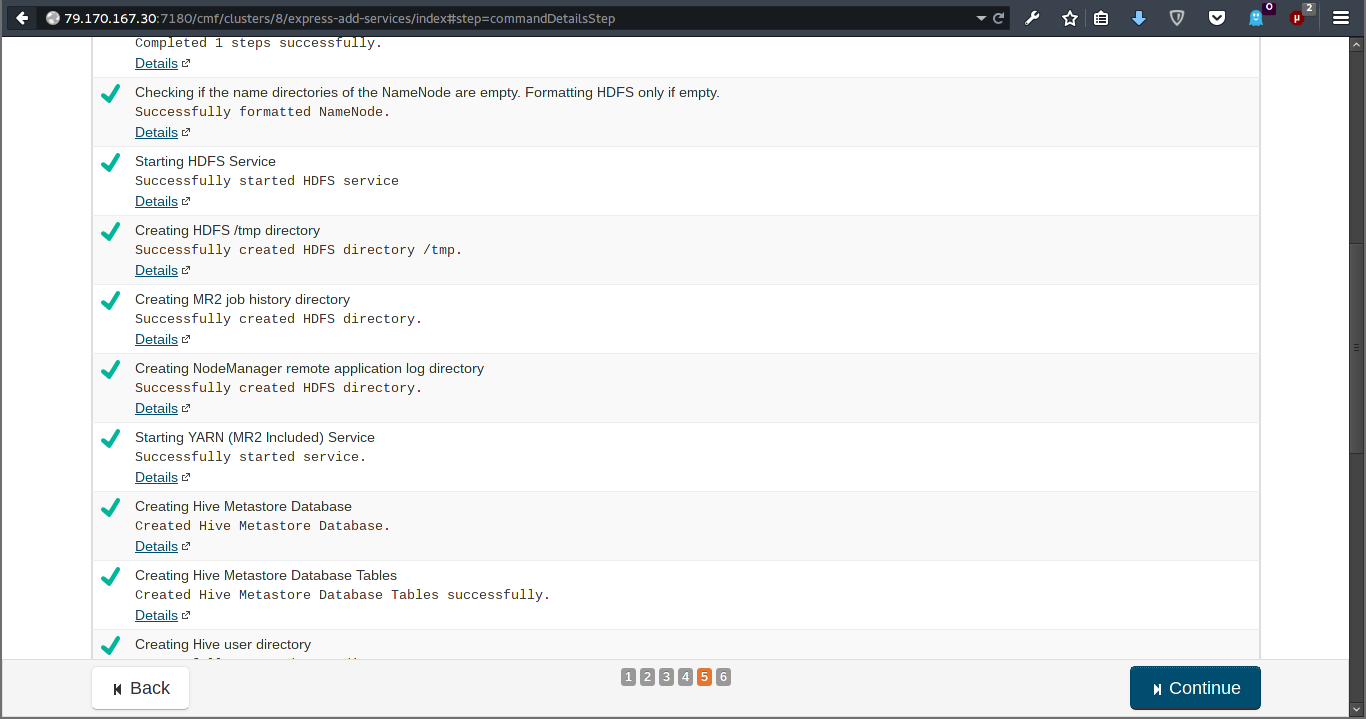
\includegraphics[width=1.0\textwidth]{image-036}
    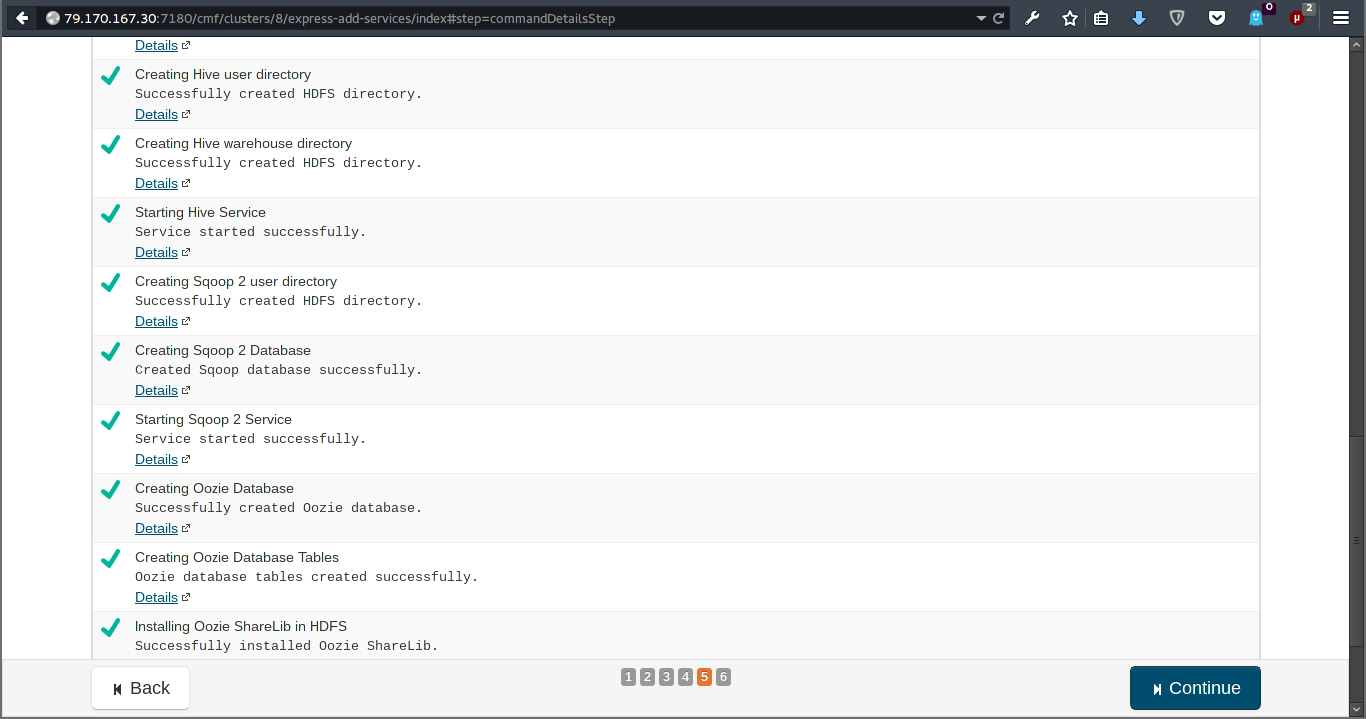
\includegraphics[width=1.0\textwidth]{image-037}
\end{figure}

\newpage

\begin{figure}[ht!]
    \center
    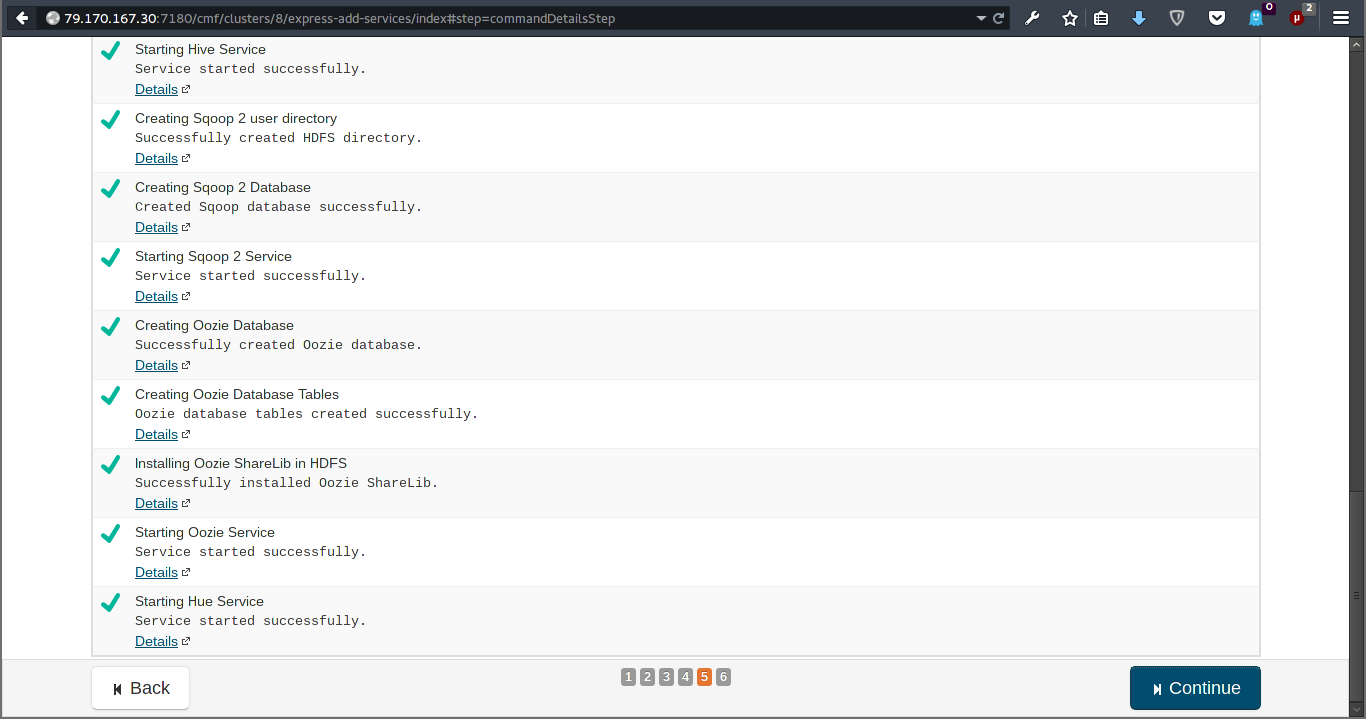
\includegraphics[width=1.0\textwidth]{image-038}
    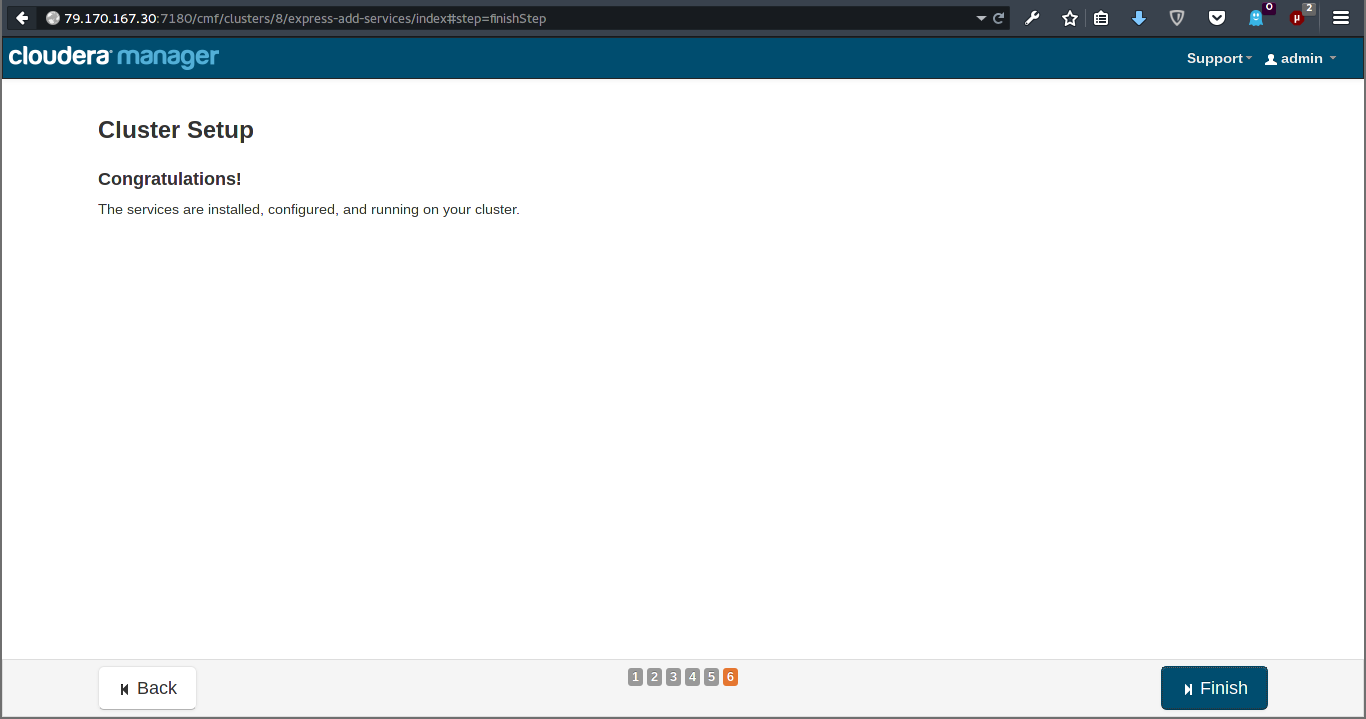
\includegraphics[width=1.0\textwidth]{image-039}
\end{figure}

\newpage

\section{Проверка работоспособности}
Для проверки работоспособности сконфигурированного кластера произведём тестовый запуск Hadoop, но для 
начала нужно произвести подготовку. Для этого создадим пользователя, через которого будем производить 
работу с HDFS и Hadoop, и установим ему пароль.
\begin{lstlisting}
$ sudo useradd -g hduser hduser
$ sudo passwd hduser
\end{lstlisting}
Создадим каталог пользователя в HDFS
\begin{lstlisting}
$ sudo -u hdfs hadoop fs -mkdir /user/hduser/
\end{lstlisting}
Сменим права на данный каталог
\begin{lstlisting}
$ sudo -u hdfs hadoop fs -chown hduser /user/hduser
\end{lstlisting}
Теперь можно использовать данного пользователя для работы с HDFS.
\begin{lstlisting}
$ su hduser
\end{lstlisting}
Создадим каталог для тестовых данных
\begin{lstlisting}
$ hadoop fs -mkdir /user/hduser/input
\end{lstlisting}
И разместим данные в нём
\begin{lstlisting}
$ hadoop fs -put /etc/hadoop/conf/*.xml /user/hduser/input 
\end{lstlisting}
Далее можно запускать Hadoop
\begin{lstlisting}
$ hadoop jar /hadoop/cloudera/parcels/CDH/jars/\
   hadoop-mapreduce-examples-2.6.0-cdh5.4.4.jar grep /user/hduser/input /user/hduser/output 'dfs[a-z.]+'
\end{lstlisting}
Если обработка закончилась успешно, то в каталоге \emph{/user/hduser/output} будут следующие файлы
\begin{lstlisting}
Found 2 items
-rw-r--r--   3 hduser supergroup          0 2015-07-26 13:59 /user/hduser/output/_SUCCESS
-rw-r--r--   3 hduser supergroup        390 2015-07-26 13:59 /user/hduser/output/part-r-00000
\end{lstlisting}
Со следующим содержимым
\begin{lstlisting}
$ hadoop fs -cat /user/hduser/output/*
1   dfs.hosts
1   dfs.namenode.acls.enabled
1   dfs.client.domain.socket.data.traffic
1   dfs.client.read.shortcircuit
1   dfs.blocksize
1   dfs.namenode.name.dir
1   dfs.datanode.hdfs
1   dfs.client.read.shortcircuit.skip.checksum
1   dfs.client.use.datanode.hostname
1   dfs.namenode.servicerpc
1   dfs.domain.socket.path
1   dfs.namenode.http
1   dfs.https.address
1   dfs.replication
1   dfs.https.port
1   dfs.groups
\end{lstlisting}
Если вы видите что-то похожее на это, то я вас поздравляю -- тестовый запуск произведён успешно!

\chapter{Установка дополнительного ПО}
\section{Установка программ из репозитория}
Программы из репозитория CentOS устанавливаются следующей командой
\begin{lstlisting}
$ sudo yum install <program>
\end{lstlisting}

\textbf{Maven}
\begin{lstlisting}
$ sudo wget http://repos.fedorapeople.org/repos/dchen/apache-maven/\
    epel-apache-maven.repo -O /etc/yum.repos.d/epel-apache-maven.repo
$ sudo yum install apache-maven
\end{lstlisting}
Если появляются проблемы с работой Maven, то возможно поможет изменение следующего параметра 
в пустое значение
\begin{lstlisting}
$ export M2_HOME=""
\end{lstlisting} 

\textbf{Lucene}
\begin{lstlisting}
$ sudo yum install lucene
\end{lstlisting}

\textbf{Tomcat}
\begin{lstlisting}
$ sudo yum install tomcat6
\end{lstlisting}
Запуск сервиса можно произвести любой из представленных команд
\begin{lstlisting}
$ sudo service tomcat6 start
$ sudo /etc/init.d/tomcat6 start
\end{lstlisting}

\section{Сборка Python 3 и установка дополнительных модулей}
Для сборки и установки Python 3 и pip необходимо установить некоторые дополнительная программы
\begin{lstlisting}
$ sudo yum groupinstall "Development tools"
$ sudo yum install zlib-devel bzip2-devel openssl-devel ncurses-devel \
    sqlite-devel readline-devel tk-devel gdbm-devel db4-devel libpcap-devel \
    xz-devel
\end{lstlisting}
Далее непосредственно сборка и установка
\begin{lstlisting}
$ wget http://www.python.org/ftp/python/3.3.2/Python-3.3.2.tar.bz2 -O /var/tmp/Python-3.3.2.tar.bz2
$ bzip2 -cd /var/tmp/Python-3.3.2.tar.bz2 | tar xvf -
$ cd Python-3.3.2
$ ./configure
$ make -j64
$ sudo make install
$ sudo ln -s /usr/local/bin/python3 /usr/bin/python3
\end{lstlisting}
Подробности доступны по ссылке \url{http://www.shayanderson.com/linux/install-python-3-on-centos-6-server.htm}

Далее нужно установить менеджер пакетов pip
\begin{lstlisting}
$ wget https://bitbucket.org/pypa/setuptools/raw/bootstrap/ez_setup.py
$ sudo /usr/local/bin/python3.2 ez_setup.py
$ sudo /usr/local/bin/easy_install-3.2 pip
\end{lstlisting}
Подробности доступны по ссылке \url{http://superuser.com/questions/773949/how-to-install-python-3-2-2-on-centos-6-5-amd64-preserving-its-original-python-i}

Для того чтобы python скрипты могли работать с PostgreSQL нужно установить пакет \emph{py-postgresql}
\begin{lstlisting}
$ sudo /usr/local/bin/pip py-postgresql
\end{lstlisting}

\section{Настройка vsftpd}
Установка vsftpd (Very Secure FTPD) производится из репозитория
\begin{lstlisting}
$ sudo yum install vsftpd
\end{lstlisting}
Далее редактируем следующие файлы
\begin{lstlisting}
$ sudo vim /etc/vsftpd/vsftpd.conf
anonymous_enable=NO
local_enable=YES
write_enable=NO
local_umask=044
anon_upload_enable=NO
anon_mkdir_write_enable=NO
dirmessage_enable=YES
xferlog_std_format=YES
async_abor_enable=YES
ascii_download_enable=YES
chroot_local_user=YES
chroot_list_enable=YES
ls_recurse_enable=YES
listen=YES
hide_ids=YES
anon_root=/hadoop/files
local_root=/hadoop/files
pam_service_name=vsftpd
userlist_enable=YES
userlist_file=/etc/vsftpd/ftpusers
user_config_dir=/etc/vsftpd/users/
tcp_wrappers=YES
guest_enable=YES
$ sudo vim /etc/pam.d/vsftpd
auth    required        pam_userdb.so   db=/etc/vsftpd/vsftpd_login
account required        pam_userdb.so   db=/etc/vsftpd/vsftpd_login
$ sudo vim /etc/vsftpd/logins.txt
<username-1>
<password-1>
<username-2>
<password-2>
...
\end{lstlisting}

Генерируем БД для виртуальных логинов и паролей 
\begin{lstlisting}
$ sudo db_load -T -t hash -f /etc/vsftpd/logins.txt /etc/vsftpd/vsftpd_login.db
$ sudo rm /etc/vsftpd/logins.txt
$ sudo chmod 600 /etc/vsftpd/vsftpd_login.db
\end{lstlisting}

Добавляем в автозапуск и запускаем
\begin{lstlisting}
$ sudo chkconfig vsftpd on
$ sudo service vsftpd start
\end{lstlisting}

Для проверки работоспособности можно использовать ftp
\begin{lstlisting}
$ ftp localhost
\end{lstlisting}

\section{Сборка Moses}
\subsection{Сборка необходимых инструментов}
Все действия в основном происходят в каталоге \emph{/hadoop/tmp/}. Дальнейшие действия являются 
адаптацией этих \url{http://www.statmt.org/moses/?n=Moses.Baseline} и 
\url{http://www.statmt.org/moses/?n=Development.GetStarted} мануалов.

Добавляем репозиторий пакетов в систему и устаналиваем boost
\begin{lstlisting}
$ sudo wget http://repo.enetres.net/enetres.repo -O /etc/yum.repos.d/enetres.repo
$ sudo yum install boost-devel
\end{lstlisting}

Клонируем репозиторий Giza++ и собираем его
\begin{lstlisting}
$ git clone https://github.com/moses-smt/giza-pp.git
$ cd giza-pp
$ make -j64
$ cd /hadoop/tmp
\end{lstlisting}

Клонируем репозиторий moses
\begin{lstlisting}
$ git clone https://github.com/moses-smt/mosesdecoder.git
\end{lstlisting}
Делаем файл bjam исполняемым и производим сборку
\begin{lstlisting}
$ chmod +x bjam
$ ./bjam -j64
\end{lstlisting}

Создаём папку для Giza++ в каталоге moses и копируем их туда
\begin{lstlisting}
$ mkdir tools
$ cp ../giza-pp/GIZA++-v2/GIZA++ ../giza-pp/GIZA++-v2/snt2cooc.out \
../giza-pp/mkcls-v2/mkcls tools
$ cd /hadoop/tmp
\end{lstlisting}

Скачиваем IRSTLM, распаковываем и производим сборку
\begin{lstlisting}
$ wget http://downloads.sourceforge.net/project/irstlm/irstlm/irstlm-5.80/irstlm-5.80.08.tgz
$ tar zxvf irstlm-5.80.08.tgz
$ cd irstlm-5.80.08/trunk
$ ./regenerate-makefiles.sh
$ ./configure --prefix=/hadoop/tmp/irstlm
$ make install
\end{lstlisting}

\subsection{Подготовка Corpus для обучения}
Создаём папку для corpus и скачиваем тренировочные данные
\begin{lstlisting}
$ mkdir corpus
$ cd corpus
$ wget http://www.statmt.org/wmt13/training-parallel-nc-v8.tgz
$ tar zxvf training-parallel-nc-v8.tgz
\end{lstlisting}

Прежде чем запускать тренировку необходимо убедиться, что в Perl установлен модуль \emph{Time/HiRes.pm}
В случае отсутствия устанавливаем следующей командой
\begin{lstlisting}
$ sudo yum install perl-Time-HiRes
\end{lstlisting}

Производим разбивка данных на токены
\begin{lstlisting}
$ ../mosesdecoder/scripts/tokenizer/tokenizer.perl -l en \
  < ./training/news-commentary-v8.fr-en.en \
  > ./news-commentary-v8.fr-en.tok.en
$ ../mosesdecoder/scripts/tokenizer/tokenizer.perl -l fr \
  < ./training/news-commentary-v8.fr-en.fr \
  > ./news-commentary-v8.fr-en.tok.fr
\end{lstlisting}

Используем truecaser
\begin{lstlisting}
$ ../mosesdecoder/scripts/recaser/train-truecaser.perl \
  --model ./truecase-model.en \
  --corpus ./news-commentary-v8.fr-en.tok.en
$ ../mosesdecoder/scripts/recaser/train-truecaser.perl \
  --model ./truecase-model.fr \
  --corpus ./news-commentary-v8.fr-en.tok.fr
\end{lstlisting}

Использование другого скрипта truecase
\begin{lstlisting}
$ ../mosesdecoder/scripts/recaser/truecase.perl \
  --model ./truecase-model.en \
  < ./news-commentary-v8.fr-en.tok.en \
  > ./news-commentary-v8.fr-en.true.en
$ ../mosesdecoder/scripts/recaser/truecase.perl \
  --model ./truecase-model.fr \
  < ./news-commentary-v8.fr-en.tok.fr \
  > ./news-commentary-v8.fr-en.true.fr
\end{lstlisting}

Далее производим чистку ограничивая длину предложения 80 символами
\begin{lstlisting}
$ ../mosesdecoder/scripts/training/clean-corpus-n.perl \
  ./news-commentary-v8.fr-en.true fr en \
  ./news-commentary-v8.fr-en.clean 1 80
\end{lstlisting}

\subsection{Тренировка модели}
\begin{lstlisting}
$ mkdir /hadoop/tmp/lm
$ cd /hadoop/tmp/lm
$ ../irstlm/bin/add-start-end.sh \
  < ../corpus/news-commentary-v8.fr-en.true.en \
  > news-commentary-v8.fr-en.sb.en
$ export IRSTLM=/hadoop/tmp/irstlm/
$ ../irstlm/bin/build-lm.sh -i news-commentary-v8.fr-en.sb.en \
  -t ./tmp -p -s improved-kneser-ney \
  -o news-commentary-v8.fr-en.lm.en
$ ../irstlm/bin/compile-lm --text=yes \
  news-commentary-v8.fr-en.lm.en.gz news-commentary-v8.fr-en.arpa.en
$ ../mosesdecoder/bin/build_binary \
  news-commentary-v8.fr-en.arpa.en news-commentary-v8.fr-en.blm.en
$ mkdir ../working; cd ../working
$ nohup nice ../mosesdecoder/scripts/training/train-model.perl -root-dir train \
  -corpus ../corpus/news-commentary-v8.fr-en.clean \
  -f fr -e en -alignment grow-diag-final-and -reordering msd-bidirectional-fe \
  -lm 0:3:/hadoop/tmp/lm/news-commentary-v8.fr-en.blm.en:8 \
  -external-bin-dir ../mosesdecoder/tools/ >& training.out &
\end{lstlisting}
Теперь остаётся только ждать когда завершится тренировка (может длится очень долго).

\subsection{Запуск moses}
Запускаем moses для проверки работоспособности перевода
\begin{lstlisting}
$ ./mosesdecoder/bin/moses -f ./working/train/model/moses.ini
\end{lstlisting}
Нужно подождать пока он загрузит данные в память, а потом можно вводить текст для перевода в терминале.

Для запуска Moses в режиме сервера необходимо произвести сборку поддержкой \emph{xmlrpc-c}.

\subsection{Сборка Moses c поддержкой xmlrpc-c и irstlm}
Устанавливаем xmlrpc-c из репозитория
\begin{lstlisting}
$ sudo yum install xmlrpc-c-devel
\end{lstlisting}

Или скачиваем последнюю версию используя \emph{svn} и производим сборку
\begin{lstlisting}
$ svn checkout http://svn.code.sf.net/p/xmlrpc-c/code/advanced xmlrpc-c
$ cd xmlrpc-c
$ ./configure --prefix=/hadoop/tmp/xmlrpc
$ make install -j64
\end{lstlisting}

Теперь переходим в каталог \emph{/hadoop/tmp/mosesdecoder} и запускаем сборку следующей командой
\begin{lstlisting}
./bjam --with-irstlm=/hadoop/tmp/irstlm/ --with-xmlrpc-c=<path to xmlrpc> -j64
\end{lstlisting}
Если сборка успешна выполнена, то теперь можно запускать moses в режиме сервера.